%%%%%%%%%%%%%%%%%%%%%%%%%%%%%%%%%%%%%%%%%
% Masters/Doctoral Thesis 
% LaTeX Template
% Version 2.5 (27/8/17)
%
% This template was downloaded from:
% http://www.LaTeXTemplates.com
%
% Version 2.x major modifications by:
% Vel (vel@latextemplates.com)
%
% This template is based on a template by:
% Steve Gunn (http://users.ecs.soton.ac.uk/srg/softwaretools/document/templates/)
% Sunil Patel (http://www.sunilpatel.co.uk/thesis-template/)
%
% Template license:
% CC BY-NC-SA 3.0 (http://creativecommons.org/licenses/by-nc-sa/3.0/)
%
%%%%%%%%%%%%%%%%%%%%%%%%%%%%%%%%%%%%%%%%%

%----------------------------------------------------------------------------------------
%	PACKAGES AND OTHER DOCUMENT CONFIGURATIONS
%----------------------------------------------------------------------------------------

\documentclass[
12pt, % The default document font size, options: 10pt, 11pt, 12pt
oneside, % Two side (alternating margins) for binding by default, uncomment to switch to one side
english, % ngerman for German
singlespacing, % Single line spacing, alternatives: onehalfspacing or doublespacing
%draft, % Uncomment to enable draft mode (no pictures, no links, overfull hboxes indicated)
%nolistspacing, % If the document is onehalfspacing or doublespacing, uncomment this to set spacing in lists to single
%liststotoc, % Uncomment to add the list of figures/tables/etc to the table of contents
%toctotoc, % Uncomment to add the main table of contents to the table of contents
%parskip, % Uncomment to add space between paragraphs
% nohyperref, % Uncomment to not load the hyperref package
headsepline, % Uncomment to get a line under the header
%chapterinoneline, % Uncomment to place the chapter title next to the number on one line
%consistentlayout, % Uncomment to change the layout of the declaration, abstract and acknowledgements pages to match the default layout
]{MastersDoctoralThesis} % The class file specifying the document structure

\usepackage{fourier} % Use the Palatino font by default
\usepackage[T1]{fontenc} % Output font encoding for international characters
\usepackage[utf8]{inputenc} % Required for inputting international characters
\usepackage{siunitx}
\usepackage{mathtools,amsthm}
\usepackage{bm}
\usepackage{algorithm}
\usepackage{algpseudocode}
\usepackage{subfig}
\usepackage{caption}
\usepackage{float}
\usepackage[inline, shortlabels]{enumitem}
\usepackage[final]{microtype}
\usepackage[backend=bibtex,style=alphabetic,natbib=true]{biblatex} % Use the bibtex backend with the authoryear citation style (which resembles APA)

\addbibresource{tesis.bib} % The filename of the bibliography

\usepackage[autostyle=true]{csquotes} % Required to generate language-dependent quotes in the bibliography

%----------------------------------------------------------------------------------------
%	MARGIN SETTINGS
%----------------------------------------------------------------------------------------

\geometry{
	paper=letterpaper, % Change to letterpaper for US letter
	inner=2.5cm, % Inner margin
	outer=3.5cm, % Outer margin
	bindingoffset=0.5cm, % Binding offset
	top=1.5cm, % Top margin
	bottom=1.5cm, % Bottom margin
	% showframe, % Uncomment to show how the type block is set on the page
}

%-----------------------------
%	Comandos especiales
%-----------------------------
\newcommand{\vecr}{\bm{r}} %% r vector
\newcommand{\vecp}{\bm{p}} %% p vector (momento)
\newcommand{\veck}{\bm{k}}
\newcommand{\nnet}{N_{\theta}(\bm{r})}
\newcommand{\rdf}{$g(r) \ $}
%%
\def\Itemautorefname{Figure}
%% For algorithm environments
\newcommand{\algorithmautorefname}{Algorithm}
%% For theorems
\newtheorem{theorem}{Theorem}
% \def\theoremautorefname{Theorem}
%%

%----------------------------------------------------------------------------------------
%	THESIS INFORMATION
%----------------------------------------------------------------------------------------

\thesistitle{Using Computational Intelligence to solve the Ornstein-Zernike equation} % Your thesis title, this is used in the title and abstract, print it elsewhere with \ttitle
\supervisor{Dr. Luis Carlos \textsc{Padierna García}\\
	Dr. Ramón \textsc{Castañeda Priego}
} % Your supervisor's name, this is used in the title page, print it elsewhere with \supname
\examiner{} % Your examiner's name, this is not currently used anywhere in the template, print it elsewhere with \examname
\degree{Master in Applied Science} % Your degree name, this is used in the title page and abstract, print it elsewhere with \degreename
\author{Edwin Armando Bedolla Montiel} % Your name, this is used in the title page and abstract, print it elsewhere with \authorname
\addresses{} % Your address, this is not currently used anywhere in the template, print it elsewhere with \addressname

\subject{Physical Sciences} % Your subject area, this is not currently used anywhere in the template, print it elsewhere with \subjectname
\keywords{} % Keywords for your thesis, this is not currently used anywhere in the template, print it elsewhere with \keywordnames
\university{\href{https://ugto.mx}{Universidad de Guanajuato}} % Your university's name and URL, this is used in the title page and abstract, print it elsewhere with \univname
\department{\href{}{University of Guanajuato}} % Your department's name and URL, this is used in the title page and abstract, print it elsewhere with \deptname
\group{\href{}{Science and Engineering Division}} % Your research group's name and URL, this is used in the title page, print it elsewhere with \groupname
\faculty{\href{}{Science and Engineering Division}} % Your faculty's name and URL, this is used in the title page and abstract, print it elsewhere with \facname

\AtBeginDocument{
\hypersetup{pdftitle=\ttitle} % Set the PDF's title to your title
\hypersetup{pdfauthor=\authorname} % Set the PDF's author to your name
\hypersetup{pdfkeywords=\keywordnames} % Set the PDF's keywords to your keywords
}

\begin{document}

\frontmatter % Use roman page numbering style (i, ii, iii, iv...) for the pre-content pages

\pagestyle{plain} % Default to the plain heading style until the thesis style is called for the body content

%----------------------------------------------------------------------------------------
%	TITLE PAGE
%----------------------------------------------------------------------------------------

\begin{titlepage}
\begin{center}

\vspace*{.035\textheight}
{\scshape\LARGE \univname\par}\vspace{1.5cm} % University name
\textsc{\Large Master's Thesis}\\[0.5cm] % Thesis type

\HRule \\[0.4cm] % Horizontal line
{\huge \bfseries \ttitle\par}\vspace{0.4cm} % Thesis title
\HRule \\[1.5cm] % Horizontal line
 
\begin{minipage}[t]{0.4\textwidth}
\begin{flushleft} \large
\emph{Author:}\\
\href{}{\authorname} % Author name - remove the \href bracket to remove the link
\end{flushleft}
\end{minipage}
\begin{minipage}[t]{0.4\textwidth}
\begin{flushright} \large
\emph{Supervisor:} \\
\href{}{\supname} % Supervisor name - remove the \href bracket to remove the link  
\end{flushright}
\end{minipage}\\[3cm]
 
\vfill

\large \textit{A thesis submitted in fulfillment of the requirements\\ for the degree of \degreename}\\[0.3cm] % University requirement text
\textit{in the}\\[0.4cm]
\groupname\\\deptname\\[2cm] % Research group name and department name
 
\vfill

{\large \today}\\[4cm] % Date
%\includegraphics{Logo} % University/department logo - uncomment to place it
 
\vfill
\end{center}
\end{titlepage}

%----------------------------------------------------------------------------------------
%	ABSTRACT PAGE
%----------------------------------------------------------------------------------------

\begin{abstract}
\addchaptertocentry{\abstractname} % Add the abstract to the table of contents
This thesis is an exploration of the use of \emph{computational intelligence} techniques to study the numerical solution of the Ornstein-Zernike equation for simple liquids. In particular, a continuous model of the hard sphere fluid is studied. There are two main proposals in this thesis. First, the use of \emph{neural networks} as a way to parametrize closure relation when solving the Ornstein-Zernike equation. It is shown that in the case of the hard sphere fluid, the neural network approach seems to reduce to the Hypernetted Chain closure.
For the second proposal, we explore the fact that if more physics is incorporated to the closure relation, a better estimate can be obtained with the use of \emph{evoluationary optimization} techniques. When choosing the modified Verlet closure relation, and leaving a couple of free parameters to be adjusted, the results are as good as those obtained from molecular simulations. The thesis is then closed with outlooks on different ways to improve the proposals presented in the current work, as well as new ways to solve the problem using other Machine Learning techniques.
\end{abstract}

%----------------------------------------------------------------------------------------
%	ACKNOWLEDGEMENTS
%----------------------------------------------------------------------------------------

\begin{acknowledgements}
\addchaptertocentry{\acknowledgementname} % Add the acknowledgements to the table of contents
\textcolor{red}{Pendiente por redactar \dots}
\end{acknowledgements}

%----------------------------------------------------------------------------------------
%	LIST OF CONTENTS/FIGURES/TABLES PAGES
%----------------------------------------------------------------------------------------

\tableofcontents % Prints the main table of contents

% \listoffigures % Prints the list of figures

% \listoftables % Prints the list of tables

%----------------------------------------------------------------------------------------
%	THESIS CONTENT - CHAPTERS
%----------------------------------------------------------------------------------------

\mainmatter % Begin numeric (1,2,3...) page numbering

\pagestyle{thesis} % Return the page headers back to the "thesis" style

% Include the chapters of the thesis as separate files from the Chapters folder
% Uncomment the lines as you write the chapters

\chapter{Introduction}
\label{Cap1}

Since the mainstream adoption of \emph{Machine Learning} (ML) methods
on common tasks such as object recognition, computer vision,
and human-computer interactions~\cite{lecunDeepLearning2015},
scientists have tried to adopt most of these techniques to further research
in their respective fields. From drug development~\cite{redaMachineLearningApplications2020}
to genetics and biotechnology~\cite{libbrechtMachineLearningApplications2015},
multiple applications of ML to current research problems have seen
widespread interest for their generalization and automatic discovery attributes.
It is with the inspiration from these applications that physicists have attempted to use 
such methods in diverse Physics fields~\cite{carleoMachineLearningPhysical2019a,dunjkoMachineLearningArtificial2018,carrasquillaMachineLearningPhases2017a}.

Most of the attempts and successes of using ML methods in Physical sciences come from
the direct application of common ML pipelines and uses, such as \emph{classification},
\emph{regression}, and \emph{unsupervised learning}~\cite{hastieElementsStatisticalLearning2009}, just to name some.
Such is the case of the determination of the
critical point of the Ising model as means of a classification task~\cite{carrasquillaMachineLearningPhases2017a}.
Similar is the case of the use of \emph{computer vision} and \emph{deep learning} 
techniques in particle physics, which have seen great applications when dealing with 
experimental data~\cite{radovicMachineLearningEnergy2018}.
In each of the previous examples, scientists have taken the most common applications
of ML methods and have adjusted them for their respective research problems.
This has the advantage that such ML techniques have been extensively researched
and developed, so physicists know that these methods are robust and useful for
the problems they have been developed for.
However, it turns out that not all ML techniques can be readily applied to the problem
at hand, and physicists should instead try to capitalize on the Physics of the problem and
use it along with the ML method to boost its usefulness, flexibility and accuracy.

It is with this perspective that physicists have preferred to incorporate most of the 
Physics into the ML method, and thus create a new form of
\emph{physics-inspired machine learning}~\cite{karniadakisPhysicsinformedMachineLearning2021a}.
One such example is the Behler-Parrinello neural network approach for energy surfaces
in the Density Functional Theory framework~\cite{behlerGeneralizedNeuralNetworkRepresentation2007a}.
Within such proposal, Behler and Parrinello chose to use some functions whose 
definition and composition are based on the properties of the system studied, which were 
atoms and their components,
and use such information as input to a \emph{regression} scheme to approximate the
energy surface of the studied system. At the moment of publication, this approach
defined a new paradigm of ML application within the physical sciences. It was no longer
the fact that simple learning tasks were used, but by including physical descriptors
in the ML methods, new ways of obtaining the same results were found.
Not only do ML methods provide mostly the same results as the physical framework they
are modeling, they also provide solutions much faster and more efficiently~\cite{zhuPhysicsconstrainedDeepLearning2019}.

Of all the research fields within Physics, in this thesis we would like to focus
our attention to the field of \emph{condensed matter physics}, and in particular, to the
field of Liquid State Theory and Soft Matter. Before we do that, however, we should
mention briefly some of the precursors to the applications of ML to said fields.
A great review by J\"{o}rg Behler~\cite{behlerPerspectiveMachineLearning2016a}
describes in great detail some of these precursors. Most applications have dealt with
materials science, computational chemistry and chemistry, and the computational aspect
of condensed matter physics. It is within these fields that new ways of using ML methods
have been developed from various needs in research. Another prime example is the coupling
of computer simulations and ML methods, such as the work by Li \emph{et al}~\cite{liMolecularDynamicsOntheFly2015}.
In this work, whenever the quantum-mechanical information is needed it is computed with
first-principles calculations. These calculations are then added to a dataset to be used
by ML methods, which in turn are used as approximators for the computer simulation.
This approach not only efficiently uses Physics in its most pure form, but it also
adopts the ML best attributes and uses them to its advantage.
For a more complete overview of some of the most impactful applications, the
review by Bedolla \emph{et al}~\cite{bedollaMachineLearningCondensed2020}
covers these and some other important aspects of ML methods applied to
condensed matter physics.

Although these are a tiny subset of all the modified applications of ML techniques
in physical sciences research, we should note that these show an important aspect
in common between them. If we wish to assimilate the physics of the problem at hand,
variations and modifications to the common ML methods and techniques are needed. 
Exploration and testing, trial and error, are an important part of the search and 
application of ML methods to Physics research. In the case of Liquid State Theory and Soft 
Matter, we can consider that most research is still in the exploration and testing stage,
although some applications have seen great success in specific scenarios.
One such successful application is the use of \emph{Support Vector Machines}\textemdash
an explicit method useful for classication and regression based on kernels and
quadratic optimization~\cite{steinwartSupportVectorMachines2008}\textemdash
in the description of the properties of glassy dynamics~\cite{schoenholzStructuralApproachRelaxation2016}.
The reason for research in Soft Matter and ML still being part of the exploration step is 
that in Soft Matter and Liquid Theory it is hard to find suitable descriptors that 
actually tell useful information from the system or phenomena~\cite{dijkstraPredictiveModellingMachine2021a}.
As such, most of the time a descriptor-based approach might not be feasible for every 
possible system. Instead, we need to explore a diverse range of possibilities when using ML 
methods within the context of Soft Matter and Liquid Theory.

Even though most research is still exploration and testing, there have been interesting
amalgamations and developments in the fields of Soft Matter, with Liquid Theory dragging
behind. In a sense, this is expected, due to the fact that Liquid Theory might be thought
of as \emph{solved}, although there is still research done within the field.
Let us focus first on the developments of Soft Matter. Instead of referring to specific
uses of ML within Soft Matter, it is more fruitful to mention some of the research groups
that have delved deep into using ML methods in Soft Matter. The group of Marjolein
Dijkstra at Utrecht University is an excellent example. Having done impactful research
in the field of Colloidal Soft Matter~\cite{dijkstraPhaseDiagramHighly1999,leunissenIonicColloidalCrystals2005},
the group is now focusing on using all the research and knowledge built and trying to
understand the best way to enforce the physics of the systems into ML techniques.
The group has explored with \emph{evolutionary algorithms} and their uses in patchy
colloids~\cite{bianchiPredictingPatchyParticle2012}. We refer to evolutionary algorithms as
derivative-free optimization algorithms that are useful for nonlinear optimization
problems~\cite{yuIntroductionEvolutionaryAlgorithms2010}.
Unsupervised methods, such as \emph{principal component analysis}~\cite{hastieElementsStatisticalLearning2009},
have been used for choosing the best descriptors in supercooled liquids~\cite{boattiniAveragingLocalStructure2021},
as well as the detection of local structure in colloidal systems~\cite{boattiniUnsupervisedLearningLocal2019a}.
All in all, these methods simplify the process of dealing with these research problems.
ML methods make it simpler and easier to identify structure and attributes from a
system. However, it is important to note that not only do these methods make it simpler,
they can also contribute to finding new things that were previously not as obvious or easy
to see.
Another work from the group is the use of classification methods 
to identify different types of crystal phases using
a mix of supervised and unsupervised methods~\cite{hastieElementsStatisticalLearning2009},
such as in the work by van Damme \emph{et al}~\cite{vandammeClassifyingCrystalsRounded2020}.
This work is quite interesting because it is a great example of using physical descriptors,
such as bond order parameters~\cite{steinhardtBondorientationalOrderLiquids1983,lechnerAccurateDeterminationCrystal2008},
along with ML methods that actively select and distinguish between the best descriptors
for the system.

Another important group that has done several advances in the use of ML within Soft Matter
is the one lead by Thomas Truskett from the University of Texas.
Their work on the use of ML methods for inverse desing of soft materials~\cite{shermanInverseMethodsDesign2020a}
is in similar ways helping out the work by the group of Dijkstra in the same research
problem~\cite{APSAPSMarcha}.
However, the work by the Truskett group is in fact more focused on the definition and
foundations of better descriptors for soft materials and off-lattice systems~\cite{jadrichUnsupervisedMachineLearning2018}.
An important topic that the group explores is the inverse design of self-assembly
systems. \emph{Self-assembly} is the property of soft materials to order their
components, such as particles, atoms or cells, without any external interactions,
into functional structures~\cite{grzybowskiSelfassemblyCrystalsCells2009}.
In this direction, their interest is particularly focused in self-assembly and how this 
phenomena can be dealt with ML methods.
In a particular work by Lindquist \emph{et al} with the Truskett group~\cite{lindquistCommunicationInverseDesign2016},
optimization-based methods were used along with standard molecular dynamics computer
simulation methods to understand how certain materials can self-assemble.
Instead of using optimization-based methods, another work from the Truskett group
deals with probabilistic ML methods for some of the same phenomena~\cite{jadrichProbabilisticInverseDesign2017}.
The difference between both these uses is that probabilistic methods are better at dealing
with probability distributions that stem from the Statistical Mechanics description of the
problem. With the use of specialized frameworks, handling these descriptors are easier
and simpler.


%% TODO: Continuar con el hilo de la exploración en materia blanda y teoría de líquidos. Mencionar algunos de los artículos de Boattini, Dijkstra, Truskett y otros sobre Materia Blanda. En un párrafo en particular hablar sobre el resultado de Goodall-Lee sobre la ecuación de OZ, y con esto comenzar la discusión de la tesis. Al final, mencionar cómo está distribuida la tesis, los capítulos y todo eso. (2 párrafos para los artículos, un párrafo para Goodall-Lee, y un párrafo para la distribución del texto) %% Introduction
\chapter{Liquid State Theory}
\label{Cap2}

In this chapter, a brief description of Liquid State Theory is carried out. In particular, 
the focus of the chapter is to state what a liquid is, its thermodynamical properties and
how equilibrium statistical mechanics is used to understand them. Then, a description of 
The hard-sphere fluid is mentioned, which is the fundamental system studied in this work.
Then, the theory of integral equations is presented, and from this the Ornstein-Zernike 
formalism is derived. The chapter is closed with a brief description of computer simulation
methods, and in particular, of the Monte Carlo computer simulation method. Monte Carlo 
simulations are numerical schemes that make it possible to study liquids based on 
first-principles, attempting to approximate the underlying probability distribution of
the system, and with this, to obtain all the physical properties of the fluid.

\section{Equilibrium Statistical Mechanics}
\label{sec:eq-statmech}

Consider a system of $N$ spherical particles in three dimensions
where each particle is characterized by its position $\vecr$ and momentum $\vecp$.
The \emph{Hamiltonian} of the system is given by
\begin{equation}
    \mathcal{H} \left( \vecr, \vecp \right) = 
    K \left( \vecp \right) + U \left( \vecr \right)
    \label{eq:hamiltonian}
\end{equation}
with $K$ the kinetic energy and $U$ the potential energy of the system.
All together, the 6$N$ variables define a \emph{phase point} in a 6$N$-dimensional
\emph{phase space}. The state point of the system is then described by a
\emph{phase space vector} $\Gamma \left( \vecr, \vecp \right)$, however, considering that all
6$N$ particles move according to Newton's equations of motion, $\Gamma$ is
a function of time, or $\Gamma(t)$. Using this phase space vector, \emph{time averages}
can be obtained for a given observable $A$ by means of the following expression
\begin{equation}
    \left< A \right> = \lim_{t \to \infty} \frac{1}{t} 
    \int_{0}^{t} A \: \Gamma(t') \: dt'
    \label{eq:time-average}
\end{equation}
If instead the complete set of state points, also known as the \emph{ensemble} of state
poitns, is considered then the average $\left< A \right>$ can then be rewritten in
terms of this ensemble. First, we point out the following for the state point vectors.
This ensemble of state points is distributed in phase space according to a probability 
distribution that is specified by the \emph{thermodynamic ensemble.} Then, if the time 
evolution of $\Gamma(t)$ is such that all states are visited eventually, irrespective of 
its initial conditions, the system satisfies the weak ergodic
theorem~\cite{kittelElementaryStatisticalPhysics2004},
and we can now rewrite the time average in \autoref{eq:time-average} with
an \emph{ensamble average} that reads
\begin{equation}
    \left< A \right> = \sum_{\Gamma} A(\Gamma) \: \rho_{ens} (\Gamma)
    \label{eq:ensemble-average}
\end{equation}
where the sum is for all state point vectors $\Gamma$ and $\rho_{ens} (\Gamma)$
is the probability density function for the ensemble. This probability function is
a weight function for the averaging procedure and should be normalized,
\begin{equation}
    \sum_{\Gamma} \rho_{ens} (\Gamma) = 1 \, .
    \label{eq:normalized}
\end{equation}
With this information, it is now time to introduce the \emph{canonical ensemble}, which
is the main ensemble used throughout this work.

\subsection{Canonical ensemble}
The canonical ensemble is established as a system of $N$ particles in a fixed volume $V$
at temperature $T$ that can exchange energy with a heat bath. This ensemble has a
probability density function associated with it,
\begin{equation}
    \rho_{NVT} = \frac{e^{-\beta \mathcal{H}(\Gamma)}}{\sum_{\Gamma} e^{-\beta \mathcal{H}(\Gamma)}}
    \label{eq:canonical-density}
\end{equation}
where $\beta=1/k_{B} T$, with $k_{B}$ Boltzmann's constant. In the classical limit of
continuous distribution functions the denominator from \autoref{eq:canonical-density}
transform into
\begin{equation}
    Q(N,V,T) = \frac{1}{N! \, h^{3N}} \int d \vecp^{N} \, d \vecr^{N} \,
    e^{- \beta \mathcal{H} \left( \vecr^N, \vecp^N \right)}
    \label{eq:canonical-partition}
\end{equation}
which is known as the \emph{canonical partition function} or sum~\cite{huangStatisticalMechanics1987}.
Here, $h$ is an arbitrary but predetermined constant with the units of energy $\times$
time. As a side note, in the original formulation by Gibbs, the value of $h$ was set
to $h=1$~\cite{gibbsElementaryPrinciplesStatistical2014}, however, since the advent
of quantum mechanics, it is now taken to be Planck's constant~\cite{tolmanPrinciplesStatisticalMechanics1979}
in order to show a correspondence between the classical and quantum formulations.
Indeed, the integrals from \autoref{eq:canonical-partition} can be separated, and the
integral over the momentum coordinates can be carried out analitically giving,
\begin{equation}
    Q(N,V,T) = \frac{1}{N! \, \Lambda^{3N}} \int d \vecr^{N} \,
    e^{- \beta U \left( \vecr^N \right)}
    \label{eq:canonical-partition-position}
\end{equation}
with $\Lambda=\sqrt{h^2 / 2 \pi m k_{B} T}$ the thermal wavelength, also known as the
\emph{de Broglie} wavelength. This again shows a correspondence between classical
and quantum formulations. The remaining integral over the positions is called the
\emph{configuration integral},
\begin{equation}
    Z(N,V,T) = \int d \vecr^{N} \, e^{- \beta U \left( \vecr^N \right)} \, .
    \label{eq:configuration-int}
\end{equation}
Finally, we arrive at the canonical ensemble density function in the continuum limit
which is
\begin{equation}
    \rho_{NVT} = \frac{e^{- \beta U(\vecr^{N})}}{Z(N,V,T)} \, .
    \label{eq:canonical-limit}
\end{equation}
Using this probability density function, the ensemble average for an observable $A$ is
computed as
\begin{equation}
    \left< A \right> = \frac{\int e^{- \beta U(\vecr^{N})} \, A(\vecr^{N}) \, d \vecr^{N}}{Z(N,V,T)} \, .
    \label{eq:average-canonical}
\end{equation}

\section{Distribution functions}

Still, the probability density function in \autoref{eq:canonical-limit} provides far more
information from the system than necessary for the calculation of thermodynamical functions
and structure properties. Instead, a focus on a small set of particles $n \ll N$ is 
preferred, in which case a \emph{reduced probability density} is defined as
\begin{equation}
    \rho^{(n)}_{N} (\vecr^{n}) \coloneqq \frac{N!}{(N-n)!} \, \frac{1}{Z(N,V,T)}
    \int e^{- \beta U(\vecr^{N})} \, d \vecr^{(N-n)} \, ,
    \label{eq:reduced-canonical}
\end{equation}
where $\rho^{(n)}_{N} (\vecr^{n})$ is also known as the equilibrium 
$n$\emph{-particle density}.
The quantity $\rho^{(n)}_{N} (\vecr^{n}) \, d \vecr^{n}$ defines the probability of finding
$n$ particles of the system with coordinates in a volume element $d \vecr^{n}$ from the
phase space, regardless of the positions and momenta of the remaining particles.
As a result of this contraction of the probability density function, it is now possible to
provide a complete description of the \emph{structure} of a fluid, while the knowledge
of low-order particle distribution functions is sufficient to calculate thermodynamic
quantities~\cite{mcquarrieStatisticalMechanics2000}.

From the definition of the $n$-particle density in \autoref{eq:reduced-canonical}, the
normalization condition is
\begin{equation}
    \int \rho^{(n)}_{N} (\vecr^{n}) \, d \vecr^{n} = \frac{N!}{(N-n)!} \, ,
    \label{eq:normalization-reduced}
\end{equation}
and in particular, the \emph{single-particle} density is
\begin{equation}
    \int \rho^{(1)}_{N} (\vecr) \, d \vecr = N ,
    \label{eq:single-particle-density}
\end{equation}
For a homogeneous fluid, \autoref{eq:single-particle-density} is then simplified
to the following expression
\begin{equation}
    \rho^{(1)}_{N} = N / V \equiv \rho
    \label{eq:homogeneous-density}
\end{equation}
where $\rho$ is the \emph{particle number density}.

The $n$-particle distribution function $g^{(n)}_{N} (\vecr^{(n)})$ is defined in terms
of the particle densities by
\begin{equation}
    g^{(n)}_{N} (\vecr^{(n)}) \coloneqq \frac{\rho^{(n)}_{N} (\vecr_{1}, \dots , \vecr_{n})}
    {\prod_{i=1}^{n} \rho^{(1)}_{N} (\vecr_{i})} \, ,
    \label{eq:gr-def}
\end{equation}
which again for a homogeneous fluid it reduces to
\begin{equation}
    \rho^{n} g^{(n)}_{N} (\vecr^{(n)}) = \rho^{(n)}_{N} (\vecr^{n}) \, .
    \label{eq:homogenous-gr}
\end{equation}
Particle distribution functions measure the extent to which the structure of a fluid 
deviates from complete randomness~\cite{hansenTheorySimpleLiquids2013}.
If the system is also isotropic, which it shall be the consideration henceforth,
the pair distribution function $g^{(2)}_{N} (\vecr_{1}, \vecr_{2})$ is a function only
of the separation $r = r_{12} = \lvert \vecr_{2} - \vecr_{1} \rvert$;
this function is the \emph{radial distribution function}, and it is referred
to as $g(r)$ for the rest of this work.
This radial distribution function is of crucial importance in Liquid State Theory for
several reasons. First, the radial distribution function can be obtained experimentally
for liquids using X-ray diffraction, digital videomicroscopy, and light scattering
experiments~\cite{mcquarrieStatisticalMechanics2000}.
Second, thermodynamic properties of liquids can be determined using integrals that
contain the radial distribution function. Lastly, the radial distribution function can
be easily computed in computer simulations~\cite{allenComputerSimulationLiquids2017}, 
which is the standard way to obtain these quantities.

\section{Thermodynamic properties}

It was mentioned before that thermodynamics properties can be defined in terms of
distribution functions, and in particular, in terms of the radial distribution
functions~\cite{hansenTheorySimpleLiquids2013}.
It is now time to discuss such expression, and the relation between thermodynamical
quantities and the radial distribution function.

The \emph{total energy} $E$ of a system of $N$ particles can be defined in terms of the
radial distribution function as
\begin{equation}
    E = E_{ideal} + E_{excess} = \frac{3 N k_{B} T}{2} +
    \frac{N}{2} \int_{0}^{\infty} \rho \, u(r) \, g(r) \, 4 \pi r^2 \, dr
    \, ,
    \label{eq:total-energy-rdf}
\end{equation}
where $E_{ideal}$ is the ideal gas contribution, whose result comes directly from
the energy equipartition theorem~\cite{mcquarrieStatisticalMechanics2000};
$E_{excess}$ is an interaction or excess contribution that can be understood
as the interaction energy between a central particle for all the $N$ particles,
and all the neighbors located in a spherical shell of radius $r$ and thickness
$dr$. The total number of neighbors is given by $4 \pi r^2 \rho g(r) \, dr$.
The integration from $0$ to $\infty$ gives all the interaction energy, and
the factor of $1/2$ accounts for double counting of particle pairs.
The function $u(r)$ is the \emph{pairwise interaction potential} which comes
from the fact that the total potential energy $U(\vecr^{N})$ can be expressed
in terms of the individual particle interactions as follows
\begin{equation}
    U(\vecr^{N}) = \sum_{i} u_{1} (\vecr_{i}^{N}) +
    \sum_{i} \sum_{j>i} u_{2} (\vecr_{i}^{N}, \vecr_{j}^{N}) +
    \dots
    \label{eq:pairwise-energy}
\end{equation}
These kind of interactions are the most commonly studied, given that most
systems can be modeled after such interaction potentials, such as the
hard-sphere, Lennard-Jones, Yukawa~\cite{huangStatisticalMechanics1987}
and several others. The hard-sphere interaction potential will be discussed
in a later section.
In the current work, the two-particle interaction potential
$u_{2} (\vecr_{i}^{N}, \vecr_{j}^{N})$ is referred to simply as $u(r)$.

The \emph{pressure equation} is a relation between the thermodynamic pressure
$P$ and the radial distribution function, defined as
\begin{equation}
    P=P_{ideal}+P_{excess}= \frac{\rho}{\beta} - \frac{2 \pi \beta \rho}{3}
    \int_{0}^{\infty} u'(r) \, g(r) \, r^3 \, dr \, ,
    \label{eq:pressure-equation}
\end{equation}
where $P_{ideal}$ is the contribution due the ideal gas, and $P_{excess}$,
the excess pressure can be derived using classical mechanics through the
virial equation~\cite{hansenTheorySimpleLiquids2013}.

Another important quantity that must be mentioned is the
\emph{isothermal compressibility}. Its thermodynamic definition is
\begin{equation}
    \chi_{T} = - \, \frac{1}{V} { \left( \frac{\partial V}{\partial P} \right) }_{T} =
    \frac{1}{\rho} { \left( \frac{\partial \rho}{\partial P} \right) }_{T}
    \label{eq:isothermal-chi}
\end{equation}
and is a physical measure of the relative change in volume due to a change
in pressure or stress.
It can also be computed using the radial distribution function using the following
expression~\cite{hansenTheorySimpleLiquids2013}
\begin{equation}
    \frac{\chi_{T} \, \beta}{\rho} = 1 + \rho \int d \vecr \, \left[ g(r) - 1 \right]
    \, .
    \label{eq:chi-rdf}
\end{equation}
We call this the \emph{compressibility equation}, and it is a standard way of computing
the isothermal compressibility. There is an alternative definition based on integral 
equation formalism, which will be discussed in a later section.

\section{Intermolecular potentials and models}

In order to model the behavior of materials, models are chosen according to specific
physical properties. All of these models are proposals for the intermolecular potentials,
and provide a particular functional form for the potential energy $U$ of the system.
Out of all the possible interaction potentials, there is one that stands out for its
simplicity and surprising ability to generalize to complex systems. This model is
called the \emph{hard sphere model}, and shall be the topic of discussion for this
section.

The \emph{hard sphere model} is a simple pairwise interaction potential, defined as
\begin{equation}
    u_{hs} = 
    \begin{cases}
        \infty \, , &r \leq \sigma \\
        0 \, , &r > \sigma \, .
    \end{cases}
    \label{eq:hard-sphere}
\end{equation}
This interaction is a model, an approximation of the intrinsic behavior of particles.
It attempts to model the excluded volume interaction of particles, similar to what
billiards balls in three dimensions. These particles seem to hit each other only to
be separated at contact with each other. Hence, this model is by definition a
\emph{repulsive model}.
Apart from being a reference model system for the liquid
state~\cite{hansenTheorySimpleLiquids2013}, hard spheres are extremely useful in
colloid science, as mentioned in the introduction section. This is due to the fact
that is has been demonstrated that the hard sphere interaction gives rise to a
fluid-crystal phase transition around a volume fraction of 50\% of hard 
spheres~\cite{hooverMeltingTransitionCommunal1968a,gastSimpleOrderingComplex1998,roblesNoteEquationState2014a}.
This phase transition was the subject of an extensive discussion in the early
1950's and was for the first time discovered in computer
simulations~\cite{alderPhaseTransitionHard1957a}.
The relationship between this simple model and colloid science was discovered
experimentally by Pusey and van Megen~\cite{puseyPhaseBehaviourConcentrated1986},
in dense colloidal suspensions of sterically stabilized particles in a solvent.

In this work a similar potential is used, though defined differently. Looking closely
at \autoref{eq:hard-sphere}, it is straightforward to see that the potential is a
discontinuous function. In mathematical proofs and statistical mechanics frameworks,
this poses no problem. It might be hard to manipulate, mathematically speaking,
but it is possible to do so. Yet, the problem lies with the use of computer simulations.
The technical issues arise mostly in Molecular and Brownian Dynamics computer
simulations~\cite{allenComputerSimulationLiquids2017}, so a different formulation
must be employed. Computer simulations of liquids are presented in the next section.
In 2018, Báez \emph{et al}~\cite{baezUsingSecondVirial2018} used the Extended Law
of Corresponding States~\cite{valadez-perezReversibleAggregationColloidal2018}
to map the second virial coefficient of the hard sphere model to a continuous
model. By doing so, most of the dynamic and thermodynamic properties of the hard sphere
model are "passed along" to the continuous function, which in turn is suited for all
kinds of computer simulation algorithms. This new continuous function is used
throughout this work, and it is defined as follows
\begin{equation}
    u_{CP} = 
    \begin{cases}
        A \, \epsilon \left[ {\left(\frac{\sigma}{r}\right)}^{\lambda} -
        {\left(\frac{\sigma}{r}\right)}^{\lambda - 1} \right] + \epsilon \, , 
        &r < \sigma \, B \, , \\
        \hspace{1.5cm} 0 \, , &r \geq \sigma \, B \, ,
    \end{cases}
    \label{eq:cont-hs}
\end{equation}
with
\begin{equation}
    A = \lambda {\left(\frac{\lambda}{\lambda -1}\right)}^{\lambda - 1} \, ,
    \quad
    B = \left(\frac{\lambda}{\lambda -1}\right) \, .
    \label{eq:ab-params}
\end{equation}
The value of $\lambda$ is fixed to $\lambda=50$, following the finding in of
Báez \emph{et al}~\cite{baezUsingSecondVirial2018}; and the value of $\epsilon$ is
not used, instead, the reduced potential is employed, i.e., $u^{*}=u_{CP} / \epsilon$. %% Liquid State Theory
%%--------- Comandos especiales
\newcommand{\vecr}{\mathbf{r}}
\newcommand{\veck}{\mathbf{k}}
\newcommand{\nnet}{N_{\theta}(\mathbf{r})}
%%
\chapter{Neural networks as an approximation for the bridge function} % Main chapter title

\label{Cap3}

%----------------------------------------------------------------------------------------
%	SECTION 1
%----------------------------------------------------------------------------------------

Neural networks can be used as \emph{universal approximators}~\cite{hornikMultilayerFeedforwardNetworks1989, hornikApproximationCapabilitiesMultilayer1991, cybenkoApproximationSuperpositionsSigmoidal1989},
in other words, they can take the form of any continuous function for some specific
types of architectures.
In particular, it is hypothesized that a neural network might be useful as a bridge function
parametrization in the closure expression for the Ornstein-Zernike equation. If this is true,
then choosing a particular approximation can be avoided for a given interaction potential, 
and leave the choice of the bridge function to the neural network itself, while
simultaneously solving the Ornstein-Zernike equation.

In this chapter, we show in detail the methodology created to achieve such a task, and
the mathematical structure with which a neural network can be used to solve the
Ornstein-Zernike equation.
These results are compared to those obtained from computer simulations to assess the
quality of the solution.
In the appendix, the detailed algorithm used to solve the Ornstein-Zernike equation
is presented, along with a detailed computation of the gradients used for the
training scheme. Here, we shall focus only on the main results and the algorithm structure
in general.

\section{Parametrization of the bridge function}

The Ornstein-Zernike equation is given by the following expression

\begin{subequations}
    \begin{align*}
         & h(\vecr) = c(\vecr) +
        n \int_{V}
        c(\vecr^{\prime})
        h(\lvert \vecr - \vecr^{\prime} \rvert)
        d\vecr^{\prime} \label{eq:oz1} \\
         & c(\vecr)
        = \exp{\left[
                -  \beta u(\vecr)
                +  \gamma(\vecr)
                + B(\vecr)
                \right]} -
        \gamma(\vecr)
        - 1
    \end{align*}
\end{subequations}

with the already known notation for each quantity (Ref a marco teórico).

Let $\nnet$ be a neural network with weights $\theta$. The main hypothesis
of this chapter is that $\nnet$ can replace the bridge function $B(\vecr)$
in the previous equation, which will yield the following expression for
the closure relation

\begin{equation}
    c(\vecr) = \exp{\left[
            -  \beta u(\vecr)
            +  \gamma(\vecr)
            + \nnet
            \right]} -
    \gamma(\vecr)
    - 1 .
    \label{eq:parametrizacion}
\end{equation}

With this new expression, the main problem to solve is to find the weights
of $\nnet$ that can successfully solve the Ornstein-Zernike equation
for a given interaction potential, $\beta u(\vecr)$.

%----------------------------------------------------------------------------------------
%	SECTION 2
%----------------------------------------------------------------------------------------

\section{Training scheme}
Now that a parametrization is defined, a way to fit the weights of the neural network must
be devised. This new numerical scheme must also be able to solve the OZ equation, while
simultaneously finding the appropiate weights for $\nnet$.

\subsection{Cost function}
It was mentioned previously that the main problem to solve is to find the weights of
$\nnet$ that can successfully solve the Ornstein-Zernike equation
for a given interaction potential.
To solve such problem, a \textbf{cost function} must be defined, and be used as part of
a \emph{minimization} problem.

To define such a function, we consider the successive approximations obtained from the
iterative Piccard scheme to solve the OZ equation, $\{\gamma_1(\vecr), \gamma_2(\vecr), \dots, \gamma_n(\vecr)\}$.
From this, we expect to have found a solution when each approximation
is \emph{close enough} to the previous one. This can be translated into the following
cost function

\begin{equation}
    J(\theta) = \left[\gamma_{n}(\vecr; \theta) - \gamma_{n-1}(\vecr; \theta) \right]^2
    \label{eq:costo}
\end{equation}

where $\gamma_{n}(\vecr; \theta)$ is the $n$-th approximation of the indirect
correlation function, $\gamma(\vecr)$.
The notation $\gamma(\vecr; \theta)$ indicates that the function now depends implicitly
on the weights of the neural network, as seen in equation~\eqref{eq:parametrizacion}.
This means that, if the weights of $\nnet$ change, we should expect a change in the output
from the $\gamma$ function. Nevertheless, this does not mean that the indirect
correlation function itself depends explicitly, nor directly, on the weights of
$\nnet$.

Another way of looking at expression~\eqref{eq:costo} is that we require that the last 
two approximations of the $\gamma$ function in each iteration from the numerical scheme to 
be as equal as possible. This will enforce a change on the weights every time both 
approximations deviate between them.

\subsection{Optimization problem}
With a cost function at hand, an optimization problem can be defined such that the
weights of $\nnet$ will be adjusted properly.

This optimization problem is in fact an \emph{unconstrained optimization problem},
and it is defined simply as

\begin{equation}
    \begin{aligned}
         & \underset{\theta}{\text{min}}
         & & J(\theta)
    \end{aligned}
    .
    \label{eq:optimizacion}
\end{equation}

This formulation is just a search for the best values for the weights that minimize
the squared difference between successive approximations.
This optimization problem can be solved iteratively, along with the solution of the
OZ equation, which is also an iterative process.

\subsection{Weight updates}
The iterative method employed to adjust the weights of $\nnet$ is based on the
\emph{gradient descent} method~\cite{nocedalNumericalOptimization2006}.
The most general update rule for a method based on gradient descent reads

\begin{equation}
    \theta_{n+1} = \theta_n - \eta \nabla_{\theta} J(\theta) .
    \label{eq:gradiente}
\end{equation}

where $\eta$ is known as the \emph{learning rate}, and it is a hyperparameter
that controls the step size at each iteration while moving toward the minimum
of a cost function. This value needs to be \emph{tuned} accordingly, so
that the method converges properly.

Regardless of the particular expression for the weight updates, every method
based on the gradient descent method \emph{requires} the gradient information from
the cost function with respect to the weights, $\nabla_{\theta} J(\theta)$.
In this particular case, the detailed computation of the gradient is described in
the appendix~\ref{AppendixA}.
Once this information is obtained, all that is left is to build an algorithm that
can correctly use this training scheme and solve the OZ equation.

\subsection{Solving the Ornstein-Zernike equation with neural networks}
Having described all the necessary elements needed, a general layout for the solution
of the Ornstein-Zernike using neural networks is now presented.

Thus, we propose the following steps to solve the OZ using the parametrization~\eqref{eq:parametrizacion}:

\begin{enumerate}
    \item Given a particular interaction potential $\beta u(\vecr)$, equation~\eqref{eq:parametrizacion} is used to obtain the value of the direct correlation function $c(\vecr; \theta)$, which now depends implicitly on the weights of $\nnet$. In this step, an initial value for $\gamma_{n}(\vecr)$ is needed, which is initialized based on the five-point Ng methodology~\ref{AppendixA}.
    \item The newly found function $c(\vecr; \theta)$ is transformed to a reciprocal space by means of the Fourier transform yielding the new function $\hat{c}(\veck; \theta)$.
    \item Then, the full OZ equation(Ref a ec) is Fourier transformed. Using the information from the previous step, a new estimation of the indirect correlation function is obtained, $\hat{\gamma}_{n+1}(\veck; \theta)$.
    \item The Fourier transform is applied once again to return all the functions to real space. With this operation, a new estimation $\gamma_{n+1}(\vecr; \theta)$ is computed from the transformed function, $\hat{\gamma}_{n+1}(\veck; \theta)$.
    \item Both estimations, $\gamma_{n}$ and $\gamma_{n+1}$, are used to evaluate the cost function~\eqref{eq:costo}, while simultaneously computing the gradient $\nabla_{\theta} J(\theta)$.
    \item The weights $\theta$ are updated a gradient descent rule, similar to~\eqref{eq:gradiente}, and the process is repeated from step 1. In the next iteration, the initial value for the indirect correlation function will be $\gamma_{n+1}$, and a new estimation $\gamma_{n+2}$ will be obtained. This process is repeated until convergence.
\end{enumerate}

\subsection{Convergence criterion}
The procedure describe in the previous section is repeated indefinetely until convergence
is achieved. This convergence criterion is defined as follows

\begin{equation}
    \sum_{i=1}^{N} {\left( \gamma^{n+1}_{i} - \gamma^{n}_{i} \right)}^2 \leq \epsilon .
    \label{eq:tolerancia}
\end{equation}

This expression is also known as the \emph{mean squared error}~\cite{goodfellowDeepLearning2016}.
Here, we sum all the $N$ elements of the squared difference between estimates $\gamma_{n+1}$
and $\gamma_{n}$. The paramater $\epsilon \in [0,1]$ is a tolerance value that indicates an 
upper bound for the error between estimations. When the computed error is below this 
tolerance value, we consider the algorithm to have converged to a particular minimum.
Specifically, the numerical tolerance in all the experiments was fixed to be
$\epsilon = \num{1e-5}$.
This means that the weights are adjusted until the successive estimations of the $\gamma$
functions are equal between them, up to the defined tolerance $\epsilon$.

%----------------------------------------------------------------------------------------
%	SECTION 3
%----------------------------------------------------------------------------------------
\section{Implementation}
In this section we detail the most important aspects about the implementation of the
method described in the previous section. This includes the topology of the neural network,
the optimization method, and the choice of activation function. The physical parameters
as well as the computer simulations methods used to solve the OZ equation are also outlined.

\subsection{Choice of optimization algorithm}
The general rule for the weight update based on gradient descent~\eqref{eq:gradiente} was
implemented to solve the optimization problem, but numerical inconsistencies rendered this 
method unstable and convergence was almost never achieved.

To solve this issue, the \emph{Adam}~\cite{kingmaAdamMethodStochastic2017} optimization 
method was chosen. This optimization method is an excellent choice for the training
of neural networks, even more so when the gradient is expected to be \emph{sparse}, i.e.
most of the elements of the gradient itself are zeros.
The \emph{Adam} method uses several rules to adjust the descent direction of the gradient,
as well as the hyperparameters related to the acceleration mechanism of the method.
Notably, there are two important hyperparameters used by the method; $\beta_1$,
which controls the moving average of the computed gradient; and $\beta_2$, which controls
the value of the gradient squared. Both parameters are necessary for the optimal 
convergence of the algorithm.

The equations that define the optimization method are the following

\begin{align}
    m &= \beta_1 m - (1 - \beta_1) \nabla_{\theta} J(\theta) \nonumber \\
    s &= \beta_2 s + (1 - \beta_2) \nabla_{\theta} J(\theta) \odot \nabla_{\theta} J(\theta) \nonumber \\
    \hat{m} &= \frac{m}{1 - \beta_1^t} \nonumber \\
    \hat{s} &= \frac{s}{1 - \beta_2^t} \nonumber \\
    \theta &= \theta + \eta \hat{m} \oslash \sqrt{\hat{s} + \varepsilon}
    \label{eq:adam}
\end{align}

where $\odot$ is the elementwise multiplication, or Hadamard product; $\oslash$
is the elementwise division, or Hadamard division; and $\varepsilon$ is a smoothing
value to prevent division by zero.

In the results presented in this chapter, the parameters were fixed to the ones reported
as optimal in the original work~\cite{kingmaAdamMethodStochastic2017}, which are
$\beta_1=\num{0.9}$ and $\beta_2=\num{0.999}$. It is important to note that this method
has its own mechanisms to control and modify the gradients, as well as the hyperparameters.
This makes it a \emph{hands-off} method, without the need to tune the hyperparameters.
The \emph{learning rate}, $\eta$ in equation~\eqref{eq:gradiente}, was fixed to
$\eta=\num{1e-4}$ for all the experiments.

\subsection{Neural network architecture}

\begin{figure}[t]
    \includegraphics[width=\textwidth]{figuras/capitulo-3/neural-network.pdf}
    \vspace{-1.5cm}
    \caption[General schematics of a neural network.]{Cartoon of a fully connected multilayer neural network. Note that there is one \emph{hidden layer}. The circles represent the \emph{nodes} or \emph{units} used to compute the final output. These nodes are being evaluated by an activation function to account for nonlinearities. The top-most nodes that seem different from the main nodes are known as the \emph{bias} nodes. The real architecture used in this chapter is larger, with many more nodes and connections, but the topology is the same.}
    \label{fig:nn-esquema}
\end{figure}

The neural network architecture used in all the experiments is very similar to the one
shown in figure~\ref{fig:nn-esquema}, with the exception of the number of nodes in all the
layers.
Particularly, the neural network is made of \emph{three layers}, all connected among them.
There is an \emph{input} layer, one \emph{hidden} layer, and a final \emph{output} layer.
All layers have the same number of nodes, which is 4096. Additional nodes are added to the
final two layers that serve as the \emph{bias}.

All the weights must be initialized appropiately, and in this case the Glorot uniform
distribution was used~\cite{glorotUnderstandingDifficultyTraining2010}, which has proven
to be an excellent way to help the convergence of neural networks.
When using the Glorot uniform distribution, the weights are initialized as
$
\theta_{ij} \sim \mathcal{U} \left[ -\frac{6}{\sqrt{(in + out)}},
\frac{6}{\sqrt{(in + out)}} \right]
$,
where $\mathcal{U}$ is the uniform probability distribution;
$in$ represents the number of units in the input layer; and $out$ the number of
units in the output layer. All bias nodes were initialized to be zero.

The activation function used was the \emph{ReLU}~\cite{glorotDeepSparseRectifier2011}
function which has the form

\begin{equation*}
    \text{ReLU}(x) = \max{(0, x)} .
\end{equation*}

This activation function is applied to all the nodes in the layers, with the exception
of the input layer. This function was chosen due to the fact that the other most common
functions ($\tanh, \text{softmax}$, etc.) were numerically unstable in the training process 
of the neural network.

\subsection{Physical parameters and simulations}

To solve the OZ equation a cutoff radius of $r_c=7\sigma$ was used, where $\sigma$ is the
particle diameter and it was fixed to be $\sigma=1$.
The interaction potential used was the pseudo hard sphere potential (Ref a ec.), both
for the solution of the OZ equation as well as the results obtained from computer simulations.

Seven different densities were explored in the range $\phi \in [\num{0.15}, \num{0.45}]$, 
with $\Delta \phi = \num{0.05}$.
For each density value, a grid of 70 points was used to ensure convergence of the iterative
algorithm when solving for the OZ equation. This was not the case for the computer 
simulations, where such partition is not needed.

Computer simulations results were obtained using the traditional Monte Carlo simulation
method for the NVT ensemble (Ref a marco teórico). The total number of particles was 2197,
the system was equilibrated for a total of 10 million Monte Carlo steps, and the radial
distribution functions were obtained from the sampling of 7 million steps, after
the system was equilibrated. To reduce the number of computations, a cutoff radius of
half the size of the simulation box was used for the evaluation of the interaction 
potential. Periodic boundary conditions were applied accordingly. The same pseudo hard 
sphere potential (Ref a ecuación) was used, instead of the true hard sphere potential, for 
a fair comparison with the results obtained from the OZ equation.

%----------------------------------------------------------------------------------------
%	SECTION 4
%----------------------------------------------------------------------------------------
\section{Results}
It is now time to investigate the results obtained from the proposed methodology, using all the elements previously described.
The main point of discussion will be the radial distribution
function \textemdash $g(r^*)$ \textemdash for different values of densities, both in the
low and high density regimes.

\subsection{Low densities}
In this section we will deal with the low 
density values of $\phi=\numlist[list-pair-separator={\enspace\text{and}\enspace}]{0.15;0.25}$, which are shown in figures~(\ref{fig:rdf15}, \ref{fig:rdf25}).
The results show that, at low densities, the HNC and neural network approximations are
more precise than the modified Verlet approximation. Although, all
approximations seem to fall short compared to computer simulations. This is seen espcially
in the neighborhood around the second peak, which are represented in the insets from
figures~(\ref{fig:rdf15}, \ref{fig:rdf25}).
It is specially important to note that the neural network approximation is a little bit 
more precise than the HNC approximation, which can be qualitatively appraised by observing 
the estimation of the main peak in the radial distribution function. This peak can be found 
in the vicinity of $r^* = 1$. Nevertheless, it is still overestimated, which is the 
same case for the HNC approximation. However, this is not the case for the modified Verlet 
approximation, which undervalue the main peak.

It is also important to notice the functional form of $g(r^*)$. For the HNC and neural
network approximations, it appears to have the same form between approximations, and it 
might as well be the same. This would imply that, somehow, the weights of the neural network
were updated enough such that a minimum was found, and this minimum was very close to the
HNC approximation. In other words, the results suggest that the weights are very close to
zero, such that when the neural network is evaluated, the output is close to the
result obtained from the HNC approximation.
Another important aspect to observe is that this functional form is slightly different
to the one seen from computer simulations, and that the modified Verlet approximation is 
closer to the form found in the computer simulations results.

\subsection{High densities}
We now turn our attention to the high density values of
$\phi=\numlist[list-pair-separator={\enspace\text{and}\enspace}]{0.35; 0.45}$,
represented in figures~(\ref{fig:rdf35}, \ref{fig:rdf45}).
In the same spirit as before with the low densities, the HNC and neural network 
approximations are not precise when compared to computer simulations. In this case,
the modified Verlet bridge function approximation is even more precise, which was expected.
This is because the HNC approximation is a very good approximation for long range
interaction potentials (Ref faltante), whereas the modified Verlet is better suited for 
short range potentials, such as the one studied here.
In this case, modified Verlet is the most precise of the approximations used, which
can be appraised in figures~(\ref{fig:rdf35}, \ref{fig:rdf45}), where the 
main peak is well estimated by the approximation when compared to the computer simulation
results. However, the HNC and neural network approximation overestimate this property.

Further, the functional form of $g(r^*)$ computed with the neural network approximation 
is quite different to the one obtained with computer simulations. Indeed, the result
obtained is similar to the one obtained with the HNC approximation. This was also the
case for low densities. This result is important, backing the hypothesis that the
neural network might reduce to the HNC approximation.
This would imply that the neural network is in fact approximating the bridge function
$B(\vecr) \approx 0$. If we now pay attention to the modified Verlet
approximation, we can see that the modified Verlet bridge function is the most precise
out of all the set of bridge functions used. In other words, we observe that this
estimation predicts the main peak well, as can be seen when compared to the results
obtained from computer simulations.

\begin{figure}
    \centering
    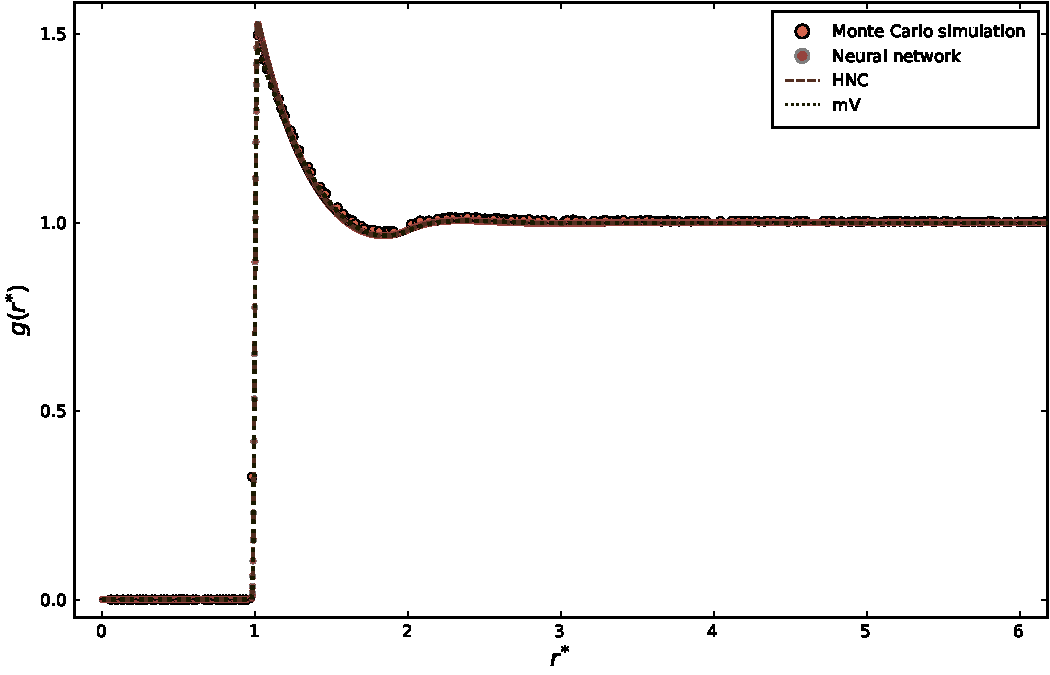
\includegraphics[width=\textwidth]{figuras/capitulo-3/comparison_p=0.15.pdf}
    \caption[Radial distribution function, $\phi=0.15$.]{The radial distribution function for density value $\phi=0.15$ obtained from computer simulations, and three different approximations:
    \begin{enumerate*}[label=(\alph*),itemjoin={,\enspace}]
        \item \emph{mV}, modified Verlet
        \item \emph{HNC}, Hypernetted Chain
        \item \emph{Neural network}, neural network approximation.
    \end{enumerate*}
    Inset shows the region close to the peak about $r^{*}=2$.
    }
    \label{fig:rdf15}
\end{figure}

\begin{figure}
    \centering
    \includegraphics[width=\textwidth]{figuras/capitulo-3/comparison_p=0.25.pdf}
    \caption[Radial distribution function, $\phi=0.25$.]{The radial distribution function for density value $\phi=0.25$ obtained from computer simulations, and three different approximations:
    \begin{enumerate*}[label=(\alph*),itemjoin={,\enspace}]
        \item \emph{mV}, modified Verlet
        \item \emph{HNC}, Hypernetted Chain
        \item \emph{Neural network}, neural network approximation.
    \end{enumerate*}
    Inset shows the region close to the peak about $r^{*}=2$.
    }
    \label{fig:rdf25}
\end{figure}

\begin{figure}
    \centering
    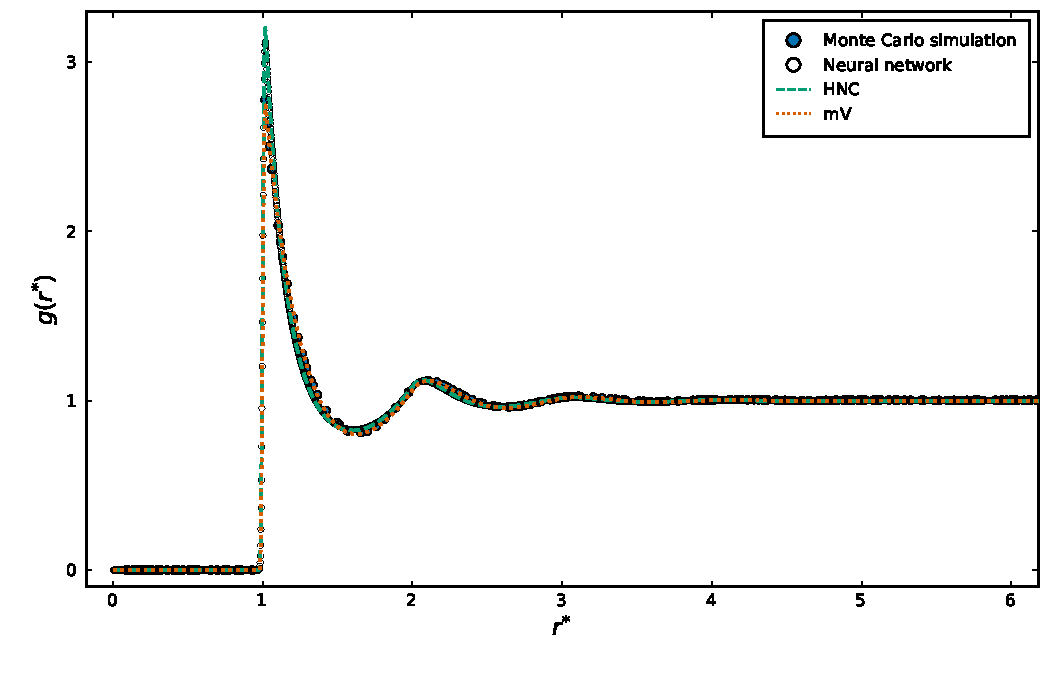
\includegraphics[width=\textwidth]{figuras/capitulo-3/comparison_p=0.35.pdf}
    \caption[Radial distribution function, $\phi=0.35$.]{The radial distribution function for density value $\phi=0.35$ obtained from computer simulations, and three different approximations:
    \begin{enumerate*}[label=(\alph*),itemjoin={,\enspace}]
        \item \emph{mV}, modified Verlet
        \item \emph{HNC}, Hypernetted Chain
        \item \emph{Neural network}, neural network approximation.
    \end{enumerate*}
    Inset shows the region close to the peak about $r^{*}=2$.
    }
    \label{fig:rdf35}
\end{figure}

\begin{figure}
    \centering
    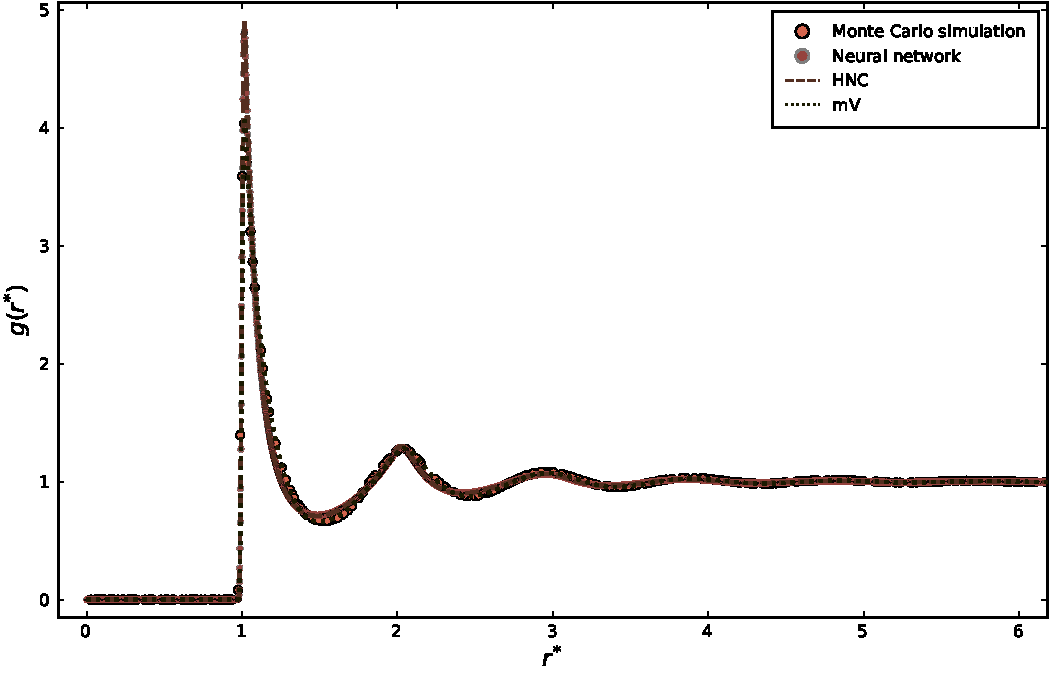
\includegraphics[width=\textwidth]{figuras/capitulo-3/comparison_p=0.45.pdf}
    \caption[Radial distribution function, $\phi=0.45$.]{The radial distribution function for density value $\phi=0.45$ obtained from computer simulations, and three different approximations:
    \begin{enumerate*}[label=(\alph*),itemjoin={,\enspace}]
        \item \emph{mV}, modified Verlet
        \item \emph{HNC}, Hypernetted Chain
        \item \emph{Neural network}, neural network approximation.
    \end{enumerate*}
    Inset shows the region close to the peak about $r^{*}=2$.
    }
    \label{fig:rdf45}
\end{figure}

\section{Discussion}
It would seem as though the neural network approximation reduces to the HNC
approximation, as seen in the results from the previous section. In this section
we shall investigate this matter in detail.
We will also continue the discussion of the results presented and try to make sense
of the training dynamics of the neural network. This is an important topic to
address due to the clear results that the neural network provides almost the same
result as the HNC approximation.

\subsection{Weight evolution of the neural network}

\begin{figure}
    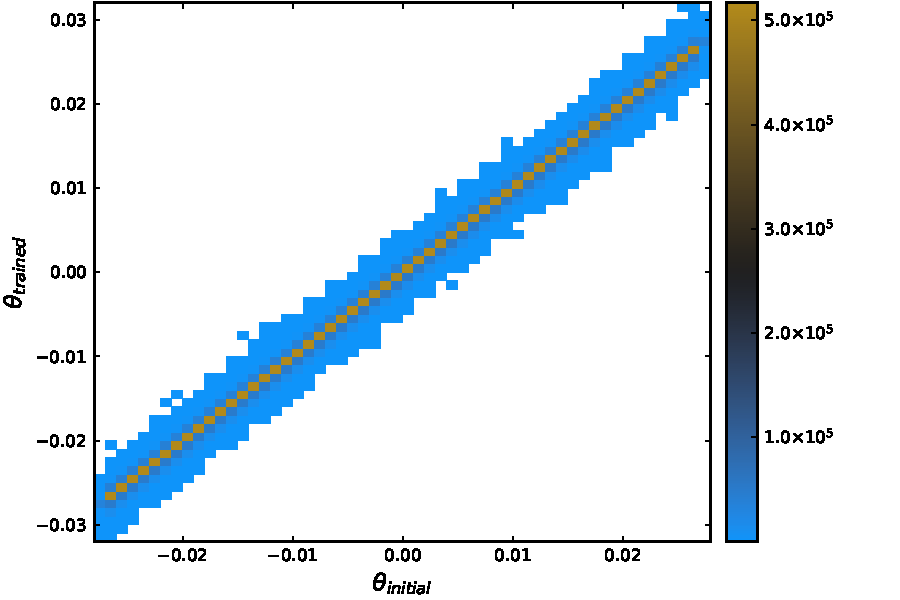
\includegraphics[width=\textwidth]{figuras/capitulo-3/weights_phi=0.15.pdf}
    \caption[Comparison between weights, $\phi=0.15$.]{Relation between the trained weights and the initial weights of $\nnet$ for the density value $\phi=0.15$. The scale on the right-hand side represents the total number of instances for the trained-initial pair of weights.} 
    \label{fig:pesos15}
\end{figure}

\begin{figure}
    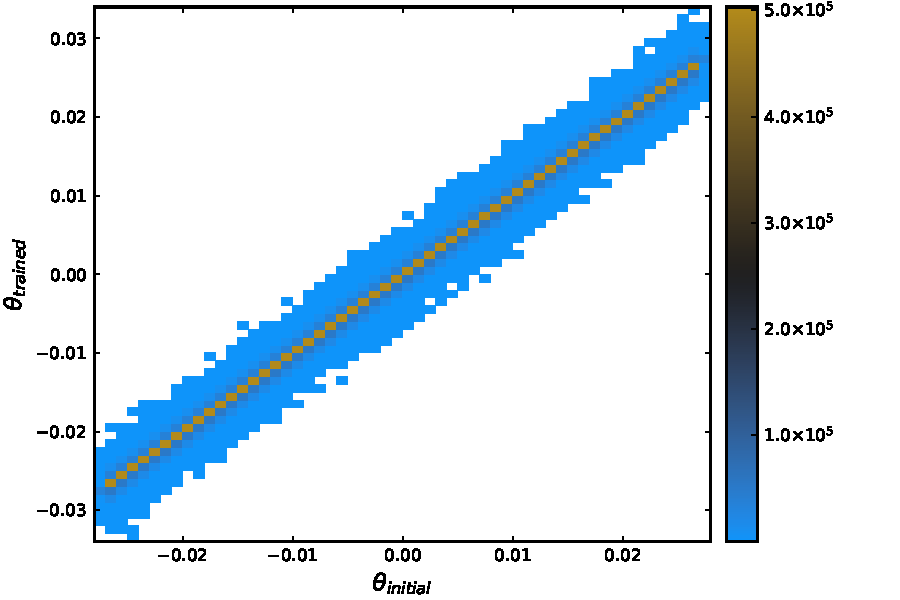
\includegraphics[width=\textwidth]{figuras/capitulo-3/weights_phi=0.25.pdf}
    \caption[Comparison between weights, $\phi=0.25$.]{Relation between the trained weights and the initial weights of $\nnet$ for the density value $\phi=0.25$. The scale on the right-hand side represents the total number of instances for the trained-initial pair of weights.}
    \label{fig:pesos25}
\end{figure}

\begin{figure}
    \includegraphics[width=\textwidth]{figuras/capitulo-3/weights_phi=0.35.pdf}
    \caption[Comparison between weights, $\phi=0.35$.]{Relation between the trained weights and the initial weights of $\nnet$ for the density value $\phi=0.35$. The scale on the right-hand side represents the total number of instances for the trained-initial pair of weights.}
    \label{fig:pesos35}
\end{figure}

\begin{figure}
    \includegraphics[width=\textwidth]{figuras/capitulo-3/weights_phi=0.45.pdf}
    \caption[Comparison between weights, $\phi=0.45$.]{Relation between the trained weights and the initial weights of $\nnet$ for the density value $\phi=0.45$. The scale on the right-hand side represents the total number of instances for the trained-initial pair of weights.}
    \label{fig:pesos45}
\end{figure}

We shall now examine the evolution of the weights $\theta$ from
$\nnet$, from the moment it was initialized to the moment its training finalized.
A histogram of this for each density value can be seen in
figures~(\ref{fig:pesos15}, \ref{fig:pesos25}, \ref{fig:pesos35}, \ref{fig:pesos45}).
We can observe that the way the weights show a diagonal represent a linear relationship 
between the initial weights, $\theta_{i}$, and the trained weights, $\theta_{t}$. In other 
words, the weights follow the linear expression
$\theta_{t} = \alpha \theta_{i} + \beta + \epsilon$, with
$\epsilon \sim \mathcal{N}(\mu, \sigma^{2})$ a normal random variable with mean
$\mu$ and variance $\sigma^2$. The noise term can be any other continuous probability 
distribution, but without loss of generality the normal distribution was chosen for
our purposes. For now, we are not interested in the values of $\alpha$ or $\beta$,
but merely on the linear relationship between them.

One thing to notice is the fact that the higher the value for the density, the larger
the variance is. If we observe the variance for the density $\phi=0.15$ in figure~\ref{fig:pesos15}
we see that the variance is small due to the fact that the blue shaded region around
the diagonal is close to it. If we now see the same figure~\ref{fig:pesos45} for the 
density value of $\phi=0.45$ we see that this shaded region is significantly larger.
This would mean that, at higher densities, the weights of $\nnet$ are more spread out
from the mean, and the neural network might have adjusted its weights to account for
different computations of the bridge function.

The most interesting part of this is the fact that the weights from initialization
do not change much throughout the training scheme, which would imply that a local minimum
has already been found. This might be the case, for the HNC is actually a solution to
the OZ equation, and solutions around this particular approximation might be as well 
solutions. This, however, does not answer the question of why the spread is larger when
higher densities are inspected.

\subsection{The Hypernetted Chain approximation as a stable minimum}
It would seem that the way the weights are updated, albeit with minimal change from its
initial values, is due to the fact of having reached a minimum already.
We must recall that the weight update and neural network training is essentially an
optimization problem~\eqref{eq:optimizacion}, and the main goal is to find a minimum
of the cost function~\eqref{eq:costo}. With the results presented so far, it might be
possible to postulate that the \emph{HNC approximation is a stable minimum} for the
neural network $\nnet$.
This would answer the question of why the weights of the neural network during training
explored in the previous section did not change very much throughout the numerical scheme.
Because if we have already found a minimum, the optimization algorithm might end up
oscillating in the proximity of this value.

On the other hand, this idea could also give answer to the question of why the spread
is large for higher density values. If we pay close attention to the approximation
results for the \emph{low density} values in figure~\ref{fig:rdf15}, we can see that
although every approximation given a low accuracy estimation of the second peak as shown
in the inset, for the main peak, the neural network approximation is very accurate.
If we now observe the figure~\ref{fig:rdf45} which refers to the \emph{high density} value
we can see that the estimation is quite poor.
Let us now relate this to the weight evolution. For the \emph{low density} regime, the 
weight evolution has a \emph{lower variance}; for the \emph{high density} regime, there
is now a \emph{higher variance} in the weight evolution.
This suggests that, for \emph{lower density} values, there was no need to adjust the
weights more than shown in figure~\ref{fig:pesos15} because the approximation is accurate
enough. However, for the \emph{higher density} values, the approximation is not good enough
and the optimization method was trying to adjust the weights accordingly, even if
unsuccessfully.

\subsection{Does the neural network reduce to HNC?}
For the low density regimes, HNC is an accurate approximation for the interaction potential.
Hence, the neural network is an accurate approximation. On the contrary, for high density
regimes, both approximation fail to provide an accurate solution.

If, in fact, the neural network is oscillating about zero (the HNC approximation), then
it makes sense that both estimations give the results observed. Yet, we cannot gaurantee
by any means possible that the neural network reduces to the HNC approximation.
We only possess \emph{statistical evidence} from the training dynamics that the neural
network weights do not change much throughout its training.

This observation might shed the light into possibilities of changing the way the neural
network propagates its values and return an output.

% TODO: Hablar sobre la poca desviación de los resultados, sobre todo hacer hincapié en el hecho de que, el no moverse mucho del cero implica que HNC es un mínimo estable y por lo tanto los pesos prefieren quedarse oscilando en este valor. Por otro lado, hablar sobre la importancia de que un valor aleatorio (o función aleatoria, matrices aleatorias, algo semejante) puede aproximar una función puente, pues esto no es algo trivial. Esto significa que se pueden aproximar las expansiones diagramáticas mediante procesos aleatorios, lo cual tiene implicaciones teóricas interesantes.
% TODO: El hecho de que los valores estén alejados del centro significa que la desviación de la media es grande. Esto puede implicar que, entre más cerca se esté del centro, menor es el cambio entre pesos entrenados e iniciales. Esto no da un argumento de porqué se reduce a HNC, sino que puede dar un argumento sobre la dinámica de entrenamiento. Esto puede ser el argumento de que quizás el hecho de que se queda alrededor de HNC porque es un mínimo ocasiona que los pesos no cambien demasiado al ser entrenados. %% Machine Learning
\chapter{Neural networks as an approximation for the bridge function}
\label{Cap4}

%----------------------------------------------------------------------------------------
%	SECTION 1
%----------------------------------------------------------------------------------------

Neural networks can be used as \emph{universal approximators},
i.e., they can take the form of any continuous function if and only if the conditions of the
universal approximation theorem hold (see \autoref{sec:approximation-thm}).
The aim of this chapter is to explore the hypothesis that a neural network might be 
useful as a bridge function parametrization in the closure expression for the 
Ornstein-Zernike equation~\cite{hansenTheorySimpleLiquids2013}.
If this is true, then choosing a particular approximation can be avoided for a given 
interaction potential, and leave the choice of the bridge function to the neural network 
itself, while simultaneously solving for the Ornstein-Zernike equation. It is intended to
explore the implications of two inquiries:

\begin{enumerate}[(a)]
    \item Is it possible to solve the Ornstein-Zernike equation using a neural network?
    \item If it is indeed possible, how good is the quality of the approximation for the pseudo hard sphere potential~\cite{baezUsingSecondVirial2018}?
\end{enumerate}

In this chapter, we show in detail the methodology created to answer these questions, and
the mathematical structure with which a neural network can be used to solve the
Ornstein-Zernike equation.
The results obtained are compared to those from Monte Carlo computer simulations to assess 
the quality of the solution.
In the appendices (\autoref{AppendixA}, \autoref{AppendixB}), the numerical algorithm used 
to solve the Ornstein-Zernike equation
is presented, along with a detailed computation of the gradients used for the
training scheme. Here, we shall focus only on the main results and the algorithm structure
in general.

\section{Parametrization of the bridge function}

The Ornstein-Zernike formalism is given by the following coupled equations~\cite{hansenTheorySimpleLiquids2013}
\begin{equation}
    \begin{aligned}
         & h(\vecr) = c(\vecr) +
        n \int_{V}
        c(\vecr^{\prime})
        h(\lvert \vecr - \vecr^{\prime} \rvert)
        d\vecr^{\prime} \\
         & c(\vecr)
        = \exp{\left[
                -  \beta u(\vecr)
                +  \gamma(\vecr)
                + B(\vecr)
                \right]} -
        \gamma(\vecr)
        - 1 ,
    \end{aligned}
    \label{eq:oz1}
\end{equation}
with the already known notation for each quantity (\textcolor{red}{Ref a marco teórico}).

Let $\nnet$ be a neural network with weights $\theta$. The main hypothesis
of this chapter is that $\nnet$ can replace the bridge function $B(\vecr)$
in the previous equation, which will yield the following expression for
the closure relation

\begin{equation}
    c(\vecr) = \exp{\left[
            -  \beta u(\vecr)
            +  \gamma(\vecr)
            + \nnet
            \right]} -
    \gamma(\vecr)
    - 1 .
    \label{eq:parametrizacion}
\end{equation}

With this new expression, the main problem to solve is to find the weights
of $\nnet$ that can successfully solve the Ornstein-Zernike equation
for a given interaction potential, $\beta u(\vecr)$.

%----------------------------------------------------------------------------------------
%	SECTION 2
%----------------------------------------------------------------------------------------

\section{Training scheme}
Now that a parametrization is defined, a way to fit the weights of the neural network must
be devised. This new numerical scheme must also be able to solve the OZ equation, while
simultaneously finding the appropiate weights for $\nnet$.

\subsection{Cost function}
It was mentioned previously that the main problem is to find the weights of
$\nnet$ that can successfully solve the Ornstein-Zernike equation
for a given interaction potential.
To solve such a problem, a \textbf{cost function} must be defined, and be used as part of
a \emph{minimization} problem.

To define such a function, we consider the successive approximations obtained from the
iterative Piccard scheme to solve the OZ equation, $\left\{\gamma_1(\vecr), \gamma_2(\vecr), \dots, \gamma_n(\vecr)\right\}$.
From this, we expect to have found a solution when each approximation
is \emph{close enough} to the previous one. This can be translated into the following
cost function
\begin{equation}
    J(\theta) = \left[\gamma_{n}(\vecr, \theta) - \gamma_{n-1}(\vecr, \theta) \right]^2 ,
    \label{eq:costo}
\end{equation}
where $\gamma_{n}(\vecr, \theta)$ is the $n$-th approximation of the indirect
correlation function, $\gamma(\vecr)$.
The notation $\gamma(\vecr, \theta)$ indicates that the function now depends
on the weights of the neural network, as seen in \autoref{eq:parametrizacion}.
This means that, if the weights of $\nnet$ change, we should expect a change in the output
from the $\gamma$ function.

Another way of looking at \autoref{eq:costo} is that we require that the last 
two approximations of the $\gamma$ function in each iteration from the numerical scheme to 
be equal within a tolerance value, or upper bound. This will enforce a change on the 
weights every time both approximations deviate between them.

\subsection{Optimization problem}
With a cost function at hand, an optimization problem can be defined such that the
weights of $\nnet$ will be adjusted properly.

This optimization problem is in fact an \emph{unconstrained optimization problem},
and it is defined simply as

\begin{equation}
    \begin{aligned}
         & \underset{\theta \in \mathbb{R}^n}{\text{min}}
         & & J(\theta) .
    \end{aligned}
    \label{eq:optimizacion}
\end{equation}

This formulation is just a search for the best values of the weights that minimize
the squared difference between successive approximations. We denote these optimal values
as the \emph{minimizer}, or $\theta^{*}$, such that $J(\theta^{*})$ is a minimum.
This optimization problem can be solved iteratively, along with the solution of the
OZ equation, whose procedure to get a solution is also through an iterative process.

\subsection{Weight updates}
The iterative method employed to adjust the weights of $\nnet$ is based on the
\emph{gradient descent} method~\cite{nocedalNumericalOptimization2006}.
The most general update rule for a method based on gradient descent reads~\cite{goodfellowDeepLearning2016}
\begin{equation}
    \theta_{n+1} = \theta_n - \eta \nabla_{\theta} J(\theta) ,
    \label{eq:gradiente}
\end{equation}
where $\eta$ is known as the \emph{learning rate}, and it is a hyperparameter
that controls the step size at each iteration while moving toward the minimum
of a cost function. This value needs to be \emph{tuned} accordingly, so
that the method converges properly. By tuning the parameter we mean that this value
should change until the numerical scheme is stable enough, or provides the best
possible answer to the optimization problem.

Regardless the particular expression for the weight updates, every method
based on the gradient descent method \emph{requires} the gradient information from
the cost function with respect to the weights, $\nabla_{\theta} J(\theta)$.
In this particular case, the detailed computation of the gradient is described in
the \autoref{AppendixA}.
Once this information is obtained, all that is left is to build an algorithm that
can correctly use this training scheme and solve the OZ equation.

\subsection{Solving the Ornstein-Zernike equation with neural networks}
\label{subsec:oz-solution}

Having described all the necessary elements needed, a general layout for the solution
of the Ornstein-Zernike using neural networks is now presented.

Thus, we propose the following steps to solve the OZ equation using the parametrization
described by \autoref{eq:parametrizacion}:

\begin{enumerate}
    \item Given a particular interaction potential $\beta u(\vecr)$, \autoref{eq:parametrizacion} is used to obtain the value of the direct correlation function $c(\vecr)$. In this step, an initial value for $\gamma_{n}(\vecr)$ is needed, which is initialized based on the five-point Ng methodology shown in \autoref{AppendixB}. The weights of the neural network $\nnet$ are initialized randomly. The initialization method is discussed in detail in the next section.
    \item The newly found function $c(\vecr)$ is transformed to a reciprocal space by means of the Fourier transform yielding the new function $\hat{c}(\veck)$.
    \item Then, the full OZ equation(\textcolor{red}{Ref a ec marco teórico}) is Fourier transformed. Using the information from the previous step, a new estimation of the indirect correlation function is obtained, $\hat{\gamma}_{n+1}(\veck, \theta)$.
    \item The Fourier transform is applied once again to return all the functions to real space. With this operation, a new estimation $\gamma_{n+1}(\vecr, \theta)$ is computed from the transformed function, $\hat{\gamma}_{n+1}(\veck, \theta)$.
    \item Both estimations, $\gamma_{n}$ and $\gamma_{n+1}$, are used to evaluate \autoref{eq:costo}. In this step, the gradient $\nabla_{\theta} J(\theta)$ is computed as well.
    \item The weights $\theta$ are updated using a gradient descent rule, similar to \autoref{eq:gradiente}, and the process is repeated from step 1. In the next iteration, the initial value for the indirect correlation function will be $\gamma_{n+1}$, and a new estimation $\gamma_{n+2}$ will be obtained. This process is repeated until convergence.
\end{enumerate}

\subsection{Convergence criterion}
The procedure described in the previous section is repeated indefinetely until convergence
is achieved. This convergence criterion is defined as follows

\begin{equation}
    \sum_{i=1}^{N} {\left( \gamma^{n+1}_{i} - \gamma^{n}_{i} \right)}^2 \leq \epsilon .
    \label{eq:tolerancia}
\end{equation}

This expression is also known as the \emph{mean squared error}~\cite{goodfellowDeepLearning2016}.
Here, we sum all the $N$ elements of the squared difference between estimates $\gamma_{n+1}$
and $\gamma_{n}$. The paramater $\epsilon$ is a tolerance value that indicates an 
upper bound for the error between estimations. When the computed error is below this 
tolerance value, we consider the algorithm to \emph{have converged to a particular minimum}.
This means that the weights are adjusted until the successive estimations of the $\gamma$
functions are equal between them, up to the defined tolerance $\epsilon$.
Specifically, the numerical tolerance in all the experiments was fixed to be
$\epsilon = \num{1e-5}$ to allow for a robust exploration of the search space, without being
too restrictive. When using a lower value of $\epsilon,$ it was observed that the results 
were not improving at all (data not shown).

%----------------------------------------------------------------------------------------
%	SECTION 3
%----------------------------------------------------------------------------------------
\section{Implementation}
In this section we detail the most important aspects about the implementation of the
method described in the previous section. This includes the topology of the neural network,
the optimization method, and the choice of activation function. The physical parameters
as well as the computer simulations methods used to solve the OZ equation are also outlined.

\subsection{Choice of optimization algorithm}
The general rule for the weight update based on \autoref{eq:gradiente} was
implemented to solve the optimization problem, but numerical inconsistencies rendered this 
method unstable and convergence was almost never achieved.

To solve this issue, the \emph{Adam}~\cite{kingmaAdamMethodStochastic2017} optimization 
method was chosen. This optimization method is an excellent choice for the training
of neural networks, even more when the gradient is expected to be \emph{sparse}, i.e.
most of the elements of the gradient itself are zeros.
The \emph{Adam} method uses several rules to adjust the descent direction of the gradient,
as well as the hyperparameters related to the acceleration mechanism of the method.
Notably, there are two important hyperparameters used in the method; $\beta_1$,
which controls the moving average of the computed gradient; and $\beta_2$, which controls
the value of the gradient squared~\cite{kingmaAdamMethodStochastic2017}. Both parameters 
are necessary for the optimal convergence of the algorithm.

The equations that define the optimization method are the following
\begin{equation}
    \begin{aligned}
        m_{t} &= \beta_1 m_{t-1} - (1 - \beta_1) \nabla_{\theta_{t-1}} J(\theta_{t-1}) \\
        s_{t} &= \beta_2 s_{t-1} + (1 - \beta_2) \nabla_{\theta_{t-1}} J(\theta_{t-1}) \odot \nabla_{\theta_{t-1}} J(\theta_{t-1}) \\
        \hat{m}_{t} &= \frac{m_{t}}{1 - \beta_1^t} \\
        \hat{s}_{t} &= \frac{s_{t}}{1 - \beta_2^t} \\
        \theta_{t} &= \theta_{t-1} + \eta \hat{m}_{t} \oslash \sqrt{\hat{s}_{t} + \varepsilon}
    \end{aligned}
    \label{eq:adam}
\end{equation}
where $\odot$ is the elementwise multiplication, or Hadamard product;
$\oslash$
is the elementwise division, or Hadamard division;
and $\varepsilon$ is a smoothing value to prevent division by zero~\cite{hornMatrixAnalysis2012}.
The index $t$ represents each of the updates, or iterations, done by the algorithm.

In the results presented in this chapter, the parameters were fixed to the ones reported
as optimal in the original work of the \emph{Adam}
method~\cite{kingmaAdamMethodStochastic2017}, which are
$\beta_1=\num{0.9}$ and $\beta_2=\num{0.999}$. It is important to note that this method
has its own mechanisms to control and modify the gradients, as well as the hyperparameters.
This makes it a \emph{hands-off} method, without the need to tune the hyperparameters.
The \emph{learning rate}, $\eta$ in \autoref{eq:gradiente}, was fixed to
$\eta=\num{1e-4}$ for all the experiments because when a larger value was used the 
optimization method did not converge properly, and the results were not useful to be 
presented here. In a more practical situation, the best
way to choose the value of $\eta$ is to employ \emph{grid search} and look for the value
that minimizes the error the most~\cite{hastieElementsStatisticalLearning2009}.

\subsection{Neural network topology}

\begin{figure}[t]
    \includegraphics[width=\textwidth]{figuras/capitulo-4/neural-network.pdf}
    \vspace{-1.5cm}
    \caption[General schematics of a neural network.]{Cartoon of a fully connected multilayer neural network. Note that there is one \emph{hidden layer}. The circles represent the \emph{nodes} or \emph{units} used to compute the final output. These nodes are being evaluated by an activation function to account for nonlinearities. The top-most nodes that seem different from the main nodes are known as the \emph{bias} nodes. The real topology used in this chapter is larger, with many more nodes and connections, but the topology is the same.}
    \label{fig:nn-esquema}
\end{figure}

The neural network topology used in all the experiments is identical to the one
shown in \autoref{fig:nn-esquema}, with the exception of the number of nodes in each layer.
In particular, the neural network is made of \emph{three layers} fully connected between 
them.
There is an \emph{input} layer, one \emph{hidden} layer, and a final \emph{output} layer.
All layers have the same number of nodes, which is 4096. Additional nodes are added to the
final two layers that serve as the \emph{bias} terms.

All the weights must be initialized appropiately, and in this case the Glorot uniform
distribution was used~\cite{glorotUnderstandingDifficultyTraining2010}, which has proven
to be an excellent way to help the convergence of neural networks.
When using the Glorot uniform distribution, the weights are initialized as
$
\theta_{ij} \sim \mathcal{U} \left[ -\frac{6}{\sqrt{(in + out)}},
\frac{6}{\sqrt{(in + out)}} \right]
$,
where $\mathcal{U}$ is the uniform probability distribution;
$in$ represents the number of units in the input layer; and $out$ the number of
units in the output layer. All bias nodes were initialized to be zero.

The activation function used was the \emph{ReLU}~\cite{glorotDeepSparseRectifier2011}
function, which has the form
\begin{equation*}
    \text{ReLU}(x) = \max{(0, x)} .
\end{equation*}

This activation function is applied to all the nodes in the layers, with the exception
of the input layer. This function was chosen due to the fact that the other most common
functions ($\tanh, \text{softmax}$, etc.) were numerically unstable in the training process 
of the neural network (data not shown).

\subsection{Physical parameters and simulations}

To solve the OZ equation a cutoff radius of $r_c=7\sigma$ was used, where $\sigma$ is the
particle diameter and it was fixed to be $\sigma=1$.
The interaction potential used was the pseudo hard sphere potential (\textcolor{red}{Ref a ec.}), both
for the solution of the OZ equation, as well as the results obtained from computer simulations.

Seven different densities were explored in the range $\phi \in [\num{0.15}, \num{0.45}]$, 
with $\Delta \phi = \num{0.05}$.
For each density value, a grid of 70 points was used to ensure convergence of the iterative
algorithm when solving for the OZ equation. This was not the case for the computer 
simulations, where such partition is not needed.

Computer simulations results were obtained using the traditional Monte Carlo simulation
method within the Metropolis scheme for the $NVT$ ensemble (\textcolor{red}{Ref a marco teórico}). In every experiment, the total number of particles was 2197,
the system was equilibrated for a total of 10 million Monte Carlo steps, and the radial
distribution functions were obtained from the sampling of 7 million Monte Carlo steps, after
the system was equilibrated. To reduce the number of computations, a cutoff radius of
half the size of the simulation box was used for the evaluation of the interaction 
potential. Periodic boundary conditions in all spatial dimensions were used accordingly. 
The same pseudo hard sphere potential (\textcolor{red}{Ref a ecuación}) was used, instead
of the true hard sphere potential, for a fair comparison with the results obtained from the 
OZ equation.

%----------------------------------------------------------------------------------------
%	SECTION 4
%----------------------------------------------------------------------------------------
\section{Results}
It is now time to investigate the results obtained from the proposed methodology, using all the elements previously described.
The main point of discussion will be the radial distribution
function \textemdash $g(r^*)$ \textemdash for different values of densities, both in the
low and high density regimes.

\subsection{Low densities}
In this section we will deal with the low 
density values ranging from $\phi=\numlist[list-pair-separator={\enspace\text{to}\enspace}]{0.15;0.25}$, which are shown in \autoref{fig:rdf15} and \autoref{fig:rdf25}, respectively.
The results show that, at low densities, the HNC and neural network approximations are
more precise than the modified Verlet approximation. Although at first glance, all
approximations seem to fall short compared to computer simulations. This is particularly 
noticeable in the neighborhood around the second peak, which is shown in the insets 
of \autoref{fig:rdf15} and \autoref{fig:rdf25}.
Additionally, it is important to note that the neural network approximation is slightly
more precise than the HNC approximation, which can be qualitatively appraised by observing 
the estimation of the main peak in the radial distribution function. This peak can be found 
in the vicinity of $r^* = 1$. Nevertheless, it is still overestimated, which is the 
same case for the HNC approximation. However, this is not the case for the modified Verlet 
approximation, which underestimates the main peak.

In like manner, the functional form of $g(r^*)$ is important to study closely.
For the HNC and neural network approximations, it appears to have the same form between 
both approximations, and it might as well be the same.
This would imply that, somehow, the weights of the neural network
were updated enough such that a minimum was found, and this minimum was very close to the
HNC approximation. In other words, the results suggest that the weights are very close to
zero, such that when the neural network is evaluated, the output is close to the
result obtained from the HNC approximation.
Another important aspect to observe is that this functional form is marginally different
to the one seen from computer simulations, and that the modified Verlet approximation is 
closer to the form found in the computer simulations results.

\subsection{High densities}
We now turn our attention to the high density values, namely,
$\phi=\numlist[list-pair-separator={\enspace\text{and}\enspace}]{0.35; 0.45}$,
represented in \autoref{fig:rdf35} and \ref{fig:rdf45}.
In the same spirit as before with the low densities, the HNC and neural network 
approximations are not precise when compared to computer simulations. In this case,
the modified Verlet bridge function approximation is even more precise, which was expected.
This is because the HNC approximation is a very good approximation for long range
interaction potentials (\textcolor{red}{Ref faltante}), whereas the modified Verlet is 
better suited for short range potentials, such as the one studied here.
In this case, modified Verlet is the most precise of the approximations used, which
can be inpsected in \autoref{fig:rdf35} and \autoref{fig:rdf45}, where the 
main peak is accurately estimated by the approximation when compared to Monte Carlo 
computer simulation results. However, both HNC and neural network approximations 
overestimate this quantity.

Further, the functional form of $g(r^*)$ computed with the neural network approximation 
is substantially different to the one obtained with computer simulations. Indeed, the result
obtained is similar to the one obtained with the HNC approximation, and both are imprecise 
approximations to the expected functional form; this was also the case for low densities.
This result is important, backing the hypothesis that the
neural network might reduce to the HNC approximation.
This would imply that the neural network is in fact approximating the bridge function
$B(\vecr) \approx 0$. If we now pay attention to the modified Verlet
approximation, again in \autoref{fig:rdf35} and \autoref{fig:rdf45}, 
we can see that the modified Verlet bridge function is the most precise
out of all the set of bridge functions used. In other words, we observe that this
estimation provides a precise prediction of the main peak, as can be seen when compared to 
the results obtained from computer simulations, which are almost identical.

\begin{figure}[t]
    \centering
    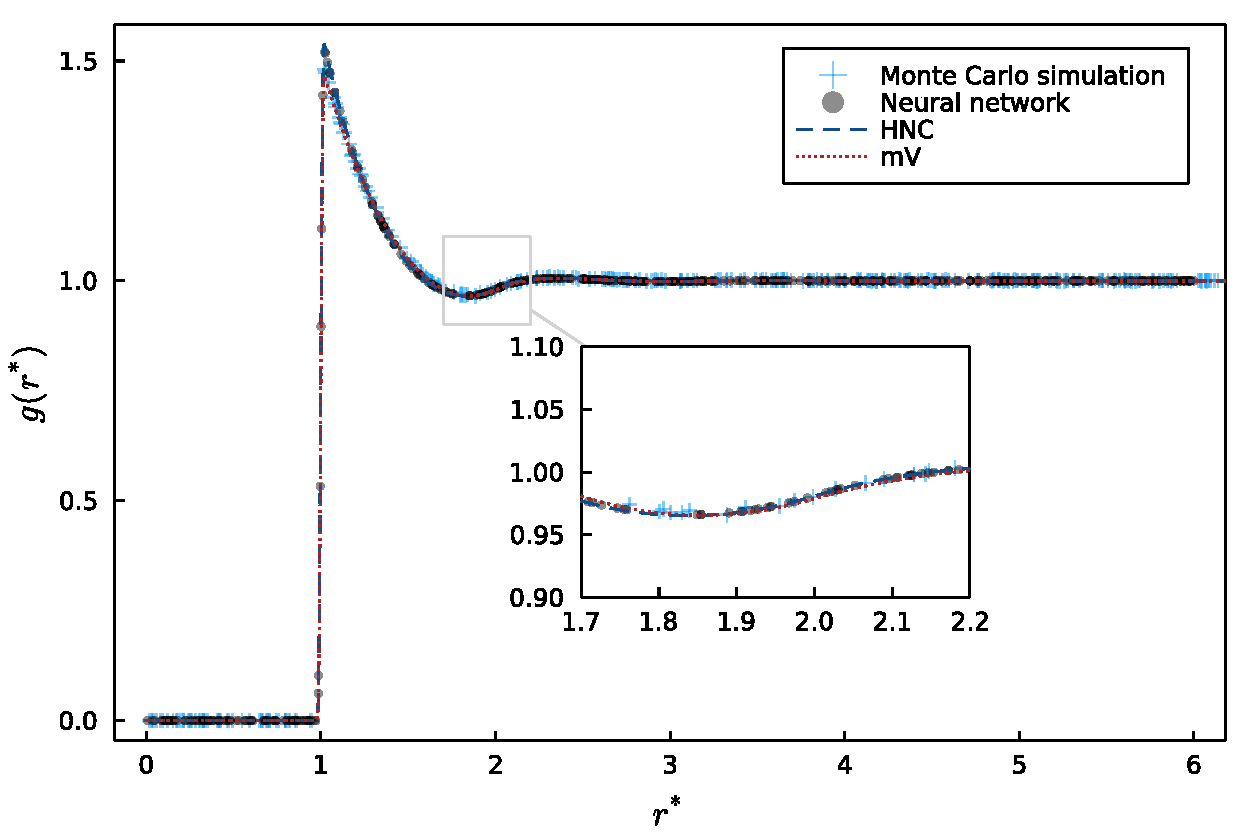
\includegraphics[width=\textwidth]{figuras/capitulo-4/comparison_p=0.15.pdf}
    \caption[Radial distribution function, $\phi=0.15$.]{Radial distribution function for $\phi=0.15$ obtained from Monte Carlo simulations, and three different approximations:
    \begin{enumerate*}[label=(\alph*),itemjoin={,\enspace}]
        \item \emph{mV}, (modified Verlet)
        \item \emph{HNC}, (Hypernetted Chain)
        \item \emph{NN}, (neural network approximation).
    \end{enumerate*}
    Inset shows the region close to the peak about $r^{*}=2$.
    }
    \label{fig:rdf15}
\end{figure}

\begin{figure}[t]
    \centering
    \includegraphics[width=\textwidth]{figuras/capitulo-4/comparison_p=0.25.pdf}
    \caption[Radial distribution function, $\phi=0.25$.]{Radial distribution function for $\phi=0.25$ obtained from Monte Carlo simulations, and three different approximations:
    \begin{enumerate*}[label=(\alph*),itemjoin={,\enspace}]
        \item \emph{mV}, (modified Verlet)
        \item \emph{HNC}, (Hypernetted Chain)
        \item \emph{NN}, (neural network approximation).
    \end{enumerate*}
    Inset shows the region close to the peak about $r^{*}=2$.
    }
    \label{fig:rdf25}
\end{figure}

\begin{figure}[t]
    \centering
    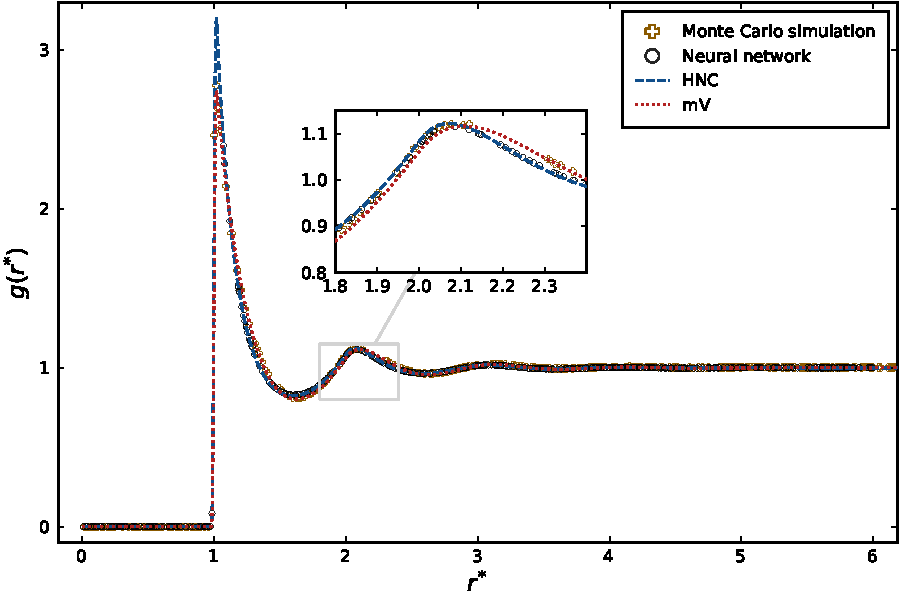
\includegraphics[width=\textwidth]{figuras/capitulo-4/comparison_p=0.35.pdf}
    \caption[Radial distribution function, $\phi=0.35$.]{Radial distribution function for $\phi=0.35$ obtained from Monte Carlo simulations, and three different approximations:
    \begin{enumerate*}[label=(\alph*),itemjoin={,\enspace}]
        \item \emph{mV}, (modified Verlet)
        \item \emph{HNC}, (Hypernetted Chain)
        \item \emph{NN}, (neural network approximation).
    \end{enumerate*}
    Inset shows the region close to the peak about $r^{*}=2$.
    }
    \label{fig:rdf35}
\end{figure}

\begin{figure}[t]
    \centering
    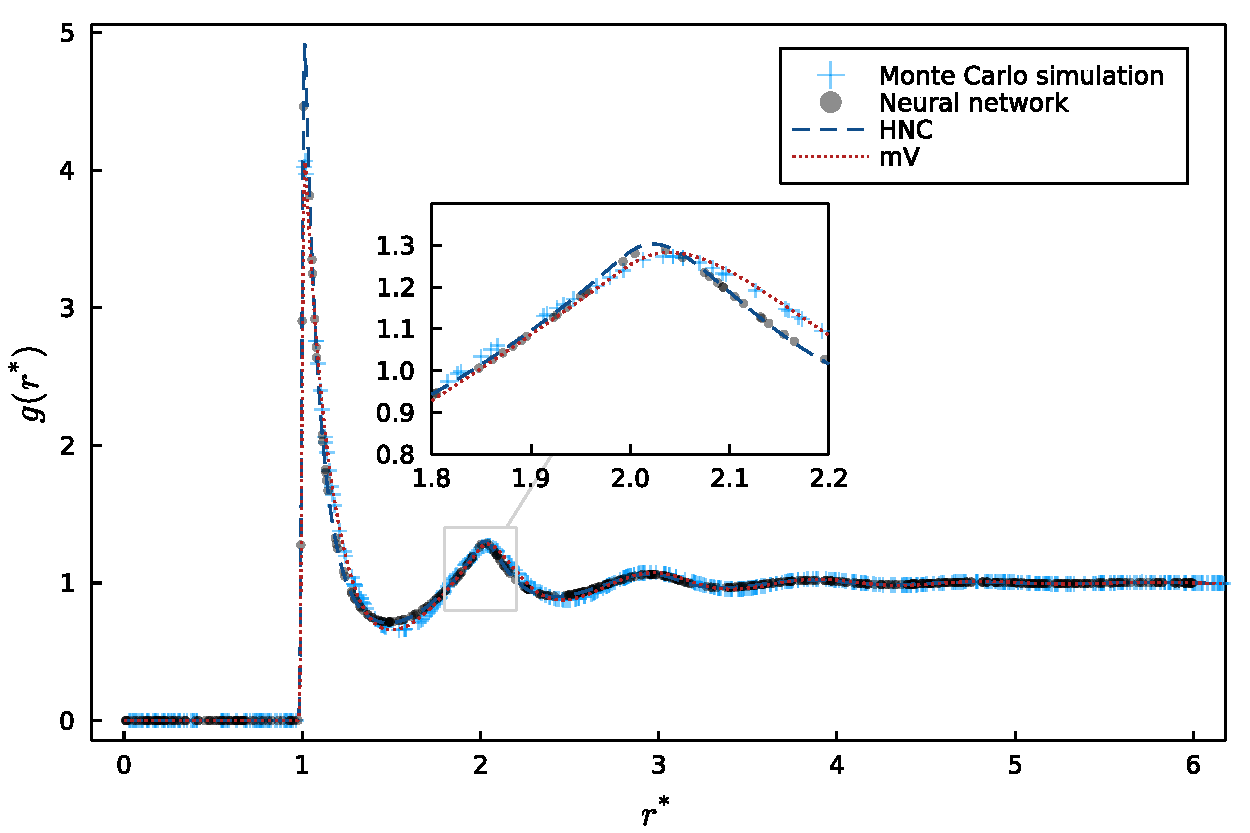
\includegraphics[width=\textwidth]{figuras/capitulo-4/comparison_p=0.45.pdf}
    \caption[Radial distribution function, $\phi=0.45$.]{Radial distribution function for $\phi=0.45$ obtained from Monte Carlo simulations, and three different approximations:
    \begin{enumerate*}[label=(\alph*),itemjoin={,\enspace}]
        \item \emph{mV}, (modified Verlet)
        \item \emph{HNC}, (Hypernetted Chain)
        \item \emph{NN}, (neural network approximation).
    \end{enumerate*}
    Inset shows the region close to the peak about $r^{*}=2$.
    }
    \label{fig:rdf45}
\end{figure}

\section{Discussion}
It would seem as though the neural network approximation reduces to the HNC
approximation, as seen in the results from the previous section. In this section
we shall investigate this matter in detail.
We will also continue the discussion of the results presented and try to make sense
of the training dynamics of the neural network. This is an important topic to
address due to the clear results that the neural network provides almost the same
result as the HNC approximation.

\subsection{Weight evolution of the neural network}

\begin{figure}[t]
    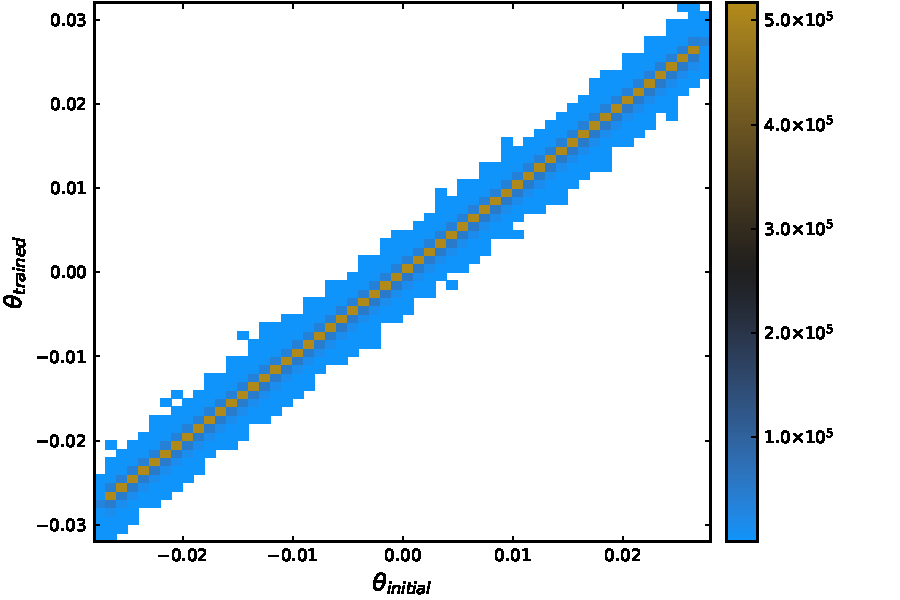
\includegraphics[width=\textwidth]{figuras/capitulo-4/weights_phi=0.15.pdf}
    \caption[Comparison between weights, $\phi=0.15$.]{Relation between the trained weights and the initial weights of $\nnet$ for $\phi=0.15$. The scale on the right-hand side represents the total number of instances for the trained-initial pair of weights.} 
    \label{fig:pesos15}
\end{figure}

We shall now examine the evolution of the weights $\theta$ from
$\nnet$, from the moment it was initialized to the moment its training finalized.
A histogram of this for the density values 
$\phi=\numlist[list-final-separator={\; \text{and} \;}]{0.15;0.25;0.35;0.45}$ 
can be seen in \autoref{fig:pesos15}, \autoref{fig:pesos25}, \autoref{fig:pesos35}, 
and \autoref{fig:pesos45}, respectively.
We can observe that the way the weights show a diagonal represent a linear relationship 
between the initial weights, $\theta_{i}$, and the trained weights, $\theta_{t}$. In other 
words, the weights follow the linear expression
$\theta_{t} = \alpha \theta_{i} + \beta + \epsilon$, with
$\epsilon \sim \mathcal{N}(\mu, \sigma^{2})$ a normal random variable with mean
$\mu$ and variance $\sigma^2$. The noise term can be any other continuous probability 
distribution, but without loss of generality the normal distribution was chosen for
our purposes. For now, we are not interested in the values of $\alpha$ or $\beta$,
but merely on the linear relationship between them.

One thing to notice is the fact that the higher the density value is, the larger
the variance turns out to be. If we observe the variance for the density
$\phi=0.15$ in \autoref{fig:pesos15}
we see that the variance is small due to the fact that the blue shaded region around
the diagonal is close to it. If we now see the same \autoref{fig:pesos45} for the 
density value of $\phi=0.45$ we observe that this shaded region is significantly larger.
This would mean that, at higher densities, the weights of $\nnet$ are more spread out
from the mean, and the neural network might have adjusted its weights to account for
different computations of the bridge function.

The most interesting part of this is the fact that the weights from initialization
do not change much throughout the training scheme, which would imply that a local minimum
has already been found. This might be the case, because HNC is actually a solution of
the OZ equation, and solutions around this particular approximation might as well be
solutions themselves.
This, however, does not answer the question of why the spread is larger when
higher densities are inspected.

\begin{figure}[t]
    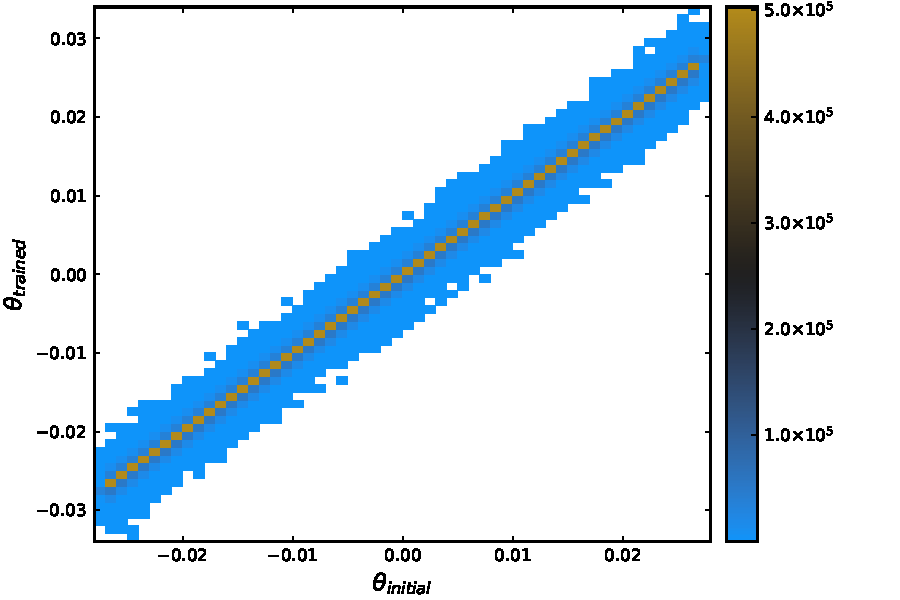
\includegraphics[width=\textwidth]{figuras/capitulo-4/weights_phi=0.25.pdf}
    \caption[Comparison between weights, $\phi=0.25$.]{Relation between the trained weights and the initial weights of $\nnet$ for $\phi=0.25$. The scale on the right-hand side represents the total number of instances for the trained-initial pair of weights.}
    \label{fig:pesos25}
\end{figure}

\subsection{The Hypernetted Chain approximation as a stable minimum}
It would seem that the way the weights are updated, albeit with minimal change from its
initial values, is due to the fact of already being near a minimum when the training starts.
We must recall that the weight update and neural network training is essentially an
optimization problem, and the main goal is to find a minimum
of the cost function in \autoref{eq:costo}. With the results presented so far, it might be
possible to postulate that the \emph{HNC approximation is a stable minimum} for the
neural network $\nnet$.
This would answer the question of why the weights of the neural network during training
explored in the previous section did not change very much throughout the numerical scheme.
Because if we have already found a minimum, the optimization algorithm might end up
oscillating in the proximity of this value.

On the other hand, this idea could also give answer to the question of why the spread
is larger for higher density values. If we pay close attention to the neural network bridge
approximation results for the \emph{low density} values in \autoref{fig:rdf15}, we can see 
that although all the bridge functions give a low accuracy estimation of the second peak as shown in the inset within the figure. However, for the main peak the neural network 
approximation is accurate.
If we now observe \autoref{fig:rdf45}, which refers to the \emph{high density} value,
we can see that the estimation is a poor one.

Let us now relate this to the weight evolution. For the \emph{low density} regime, the 
weight evolution has a \emph{lower variance}; for the \emph{high density} regime, a \emph{higher variance} is observed in the weight evolution.
This suggests that, for \emph{lower density} values, there was no need to adjust the
weights more than shown in \autoref{fig:pesos15} because the approximation is accurate
enough. However, for the \emph{higher density} values, the approximation is not good enough
and the optimization method was trying to adjust the weights accordingly, even if
unsuccessfully.
Thus, by oscillating near the value of zero, which represents the HNC bridge function,
the neural network does not need additional information and generates a bridge function 
approximation that reproduces the results from the HNC closure relation.

Having a stable minimum when training starts would mean that the neural network does not
learn enough, and will alway keep its weights tightly centered about the mean of this
minimum. Still, this implies that other minima are available for the neural network as long
as the weights are correctly initialized, or a probability distribution centered about
a particular minima is used.

\begin{figure}[t]
    \includegraphics[width=\textwidth]{figuras/capitulo-4/weights_phi=0.35.pdf}
    \caption[Comparison between weights, $\phi=0.35$.]{Relation between the trained weights and the initial weights of $\nnet$ for $\phi=0.35$. The scale on the right-hand side represents the total number of instances for the trained-initial pair of weights.}
    \label{fig:pesos35}
\end{figure}

\subsection{Does the neural network reduce to HNC?}
For the low density regimes, HNC is an accurate approximation for the interaction potential.
Hence, the neural network is an accurate approximation. On the contrary, for high density
regimes, both approximations fail to provide an accurate solution.

If the neural network is in indeed oscillating about zero (the HNC approximation), then
it makes sense that both estimations give the results observed. Yet, we cannot guarantee
by any means possible that the neural network reduces to the HNC approximation.
We only possess \emph{statistical evidence} from the training dynamics that the neural
network weights do not change much throughout its training.

This observation might shed light into possibilities of changing the way the neural
network propagates its values and return an output. For example, a modification to the
neural network topology might be in order, such that introducing important 
nonlinearities that are consistent with the physical properties of the system can yield
better results. For the case of hard spheres, the work by Malijevský and Labík~\cite{malijevskyBridgeFunctionHard1987}
shows that the bridge function has particular functional properties, such that the
bridge function is non-negative and oscillating, among others. These properties can then
be consolidated within the neural network structure and investigate if the neural network 
weights change considerably.
From this, one might expect two outcomes. Firstly, the case where the \emph{weights change},
which would indicate that adding nonlinearities according to some aspect of the interaction 
potential prove benefitial for the weight update and training dynamics.
Secondly, the case where the \emph{weights do not change}, in which case we might
be able the have stronger evidence that, regardless of the neural network structure,
this kind of approximation will have a high chance of reproducing the HNC results.
In any case, with either outcome we do not have the information to assess if the neural
network might actually be \emph{more precise} than it is in its current form.

\begin{figure}[t]
    \includegraphics[width=\textwidth]{figuras/capitulo-4/weights_phi=0.45.pdf}
    \caption[Comparison between weights, $\phi=0.45$.]{Relation between the trained weights and the initial weights of $\nnet$ for $\phi=0.45$. The scale on the right-hand side represents the total number of instances for the trained-initial pair of weights.}
    \label{fig:pesos45}
\end{figure}

Similar results were found by Goodall and Lee~\cite{a.goodallDatadrivenApproximationsBridge2021}
while using data from simulations. In this approach, a data set was built with several
correlation functions that came from physical properties of the liquid. If the data set was built
just using the indirect correlation function $\gamma(\vecr)$, the neural network trained from this data
set would yield results similar or worse to those obtained with the HNC approximation.
So, in some sense, the proposed methodology here might actually be better than a fully
data-driven methodology. However, this just makes a stronger case for the argument that,
indeed, the neural network might reduce to the HNC approximation and not have enough
information about the system to adjust the weights properly.

\subsection{Neural networks as random polynomial approximations}
An interesting result from this investigation is the fact that a random approximation
provides a solution to the OZ equation. In what way is it random? Take the weights of the
neural network to be the coefficients of some \emph{random polynomial}, i.e. a polynomial 
with coefficients that come from some probability distribution $P$. This is something that 
is not trivial on why it could work as a bridge function approximation, even if the result
is very close to the HNC approximation. This would imply that, for the probability 
distribution $P$ with some finite variance $\sigma^2$ and mean $\mu=0$, the resulting
polynomial would yield a bridge function estimation similar to the HNC closure relation.
Yet, the reason why a random approximation might be a solution to the OZ equation is not
clear.

To understand the significance of this, we must recall that the bridge function can, in 
fact, be understood as a
power series in density~\cite{hansenTheorySimpleLiquids2013},
\begin{equation}
    b(\vecr) = b^{(2)}(\vecr) \rho^2 + b^{(3)}(\vecr) \rho^3 + \cdots ,
    \label{eq:expansion-densidad}
\end{equation}
where the notation $b^{(n)}(\vecr)$ indicates the $n$-particle bridge function, i.e. the
estimation of the bridge function for $n$ interacting particles. It is specially
important to note that the coefficients $b^{(n)}(\vecr)$ are, in general, high-dimensional
integrals that are mostly \emph{intractable}. Almost always, for a given bridge function
approximation, numerical methods are in order if these coefficients are to be determined.
For instance, the work by Kwak and Kofke~\cite{kwakEvaluationBridgefunctionDiagrams2005}
uses a Monte Carlo sampling numerical method to evaluate up to $b^{(4)}(\vecr)$ 
for the hard-sphere fluid. They report that even if the numerical computation is
possible, convergence is slow and computationally costly.

Only for special cases, these coefficients can be determined in closed form, e.g.
for the Percus-Yevick approximation the value of
\[
b^{(2)}(\vecr) = -\frac{1}{2}{\left[ g_{1}(\vecr) \right]}^2
\]
is known from diagrammatic methods~\cite{hansenTheorySimpleLiquids2013}. In this
expression, $g_{1}(\vecr)$ represents the single-particle radial distribution function.

Let us now understand the role of \emph{random polynomials} and their relation to the neural
network bridge function approximation used in this investigation.
Let $p_n$ be an algebraic polynomial of the form
\begin{equation}
    p_n(z) = a_0 + a_1 z + a_2 z^2 + a_3 z^3 + \cdots + a_n z^n, \quad
    z \in \mathbb{C}
    \label{eq:random-poly}
\end{equation}
where the coefficients $a_0, a_1, \dots , a_n$ are independent real-valued random variables
with finite mean and finite variance. This kind of polynomials have found successful
applications in some areas of physics~\cite{houghZerosGaussianAnalytic2009}.
These polynomials have also been the interest of mathematical research~\cite{edelmanHowManyZeros1995}.

Now, by means of the universal approximation theorem, we can regard the neural network
as a power series similar to \autoref{eq:random-poly}. To see this more clearly, we
can think of the weights of the neural network as some coefficients of a power series,
obtained under some transformation that takes in the weights and return the coefficients
needed to build a power series.
Further, if we compare directly \autoref{eq:random-poly}
and \autoref{eq:expansion-densidad}, we can see that these expressions
are related through their coefficients, with the exception of the first two terms, implying 
that random variables might be able to give an answer to the $n$ particle bridge functions 
in the power series.

Indeed, this is a convenient way of estimating the coefficients of the bridge function,
when expressed in a power series of the density or any other correlation functions.
Although, the practical way to estimate these coefficients is to enforce thermodynamic
self-consistency. Such is the case of the work by Vompe and Martynov~\cite{vompeBridgeFunctionExpansion1994},
and the work by Tsednee and Luchko~\cite{tsedneeClosureOrnsteinZernikeEquation2019}, where
the coefficients are found through a minimization problem when the thermodynamic consistency
among different routes has been achieved.

After all, the insight of random polynomials might pave the way for a novel way of 
computing coefficients by using neural networks, or related probabilistic methods.
Even though there is no way to enforce thermodynamic self-consistency when using such
methods, it is interesting to see the striking resemblance with these approaches.
And yet, one of the downsides of this is the fact that the probability
distribution for the coefficients $a_0, a_1, \dots , a_n$ cannot be known even through the
training dynamics of the neural network. A naive way of acquiring the underlying 
probability distribution is to suppose there is
a unique probability distribution and estimate its mean and variance by maximum likelihood
estimation techniques~\cite{hastieElementsStatisticalLearning2009}.
Still, even if there could be a relation between random polynomials and the bridge 
function, there can be no guarantee that the resulting approximation is good enough, or 
that it could reproduce the physics of the problem properly.
This is just mere speculation that a deeper relationship between the neural network 
approximation and the bridge function might be exploitable through the lens of random
polynomials and probability theory.

\section{Concluding remarks}
Even though neural networks can approximate any continuous function,
it is up to the implementation that uses them
to benefit from the underlying domain knowledge of the problem to be solved. In this case,
even if the methodology created is \emph{theoretically possible}, it raises the question of
whether the neural networks are the most suitable solution for the OZ equation.
Such might be the case for the methodology presented here. After all, the results
seem to \emph{strongly suggest} that a neural network reduces to one of the classic 
approximations,
the Hypernetted Chain approximation, which is not the best approximation for all kinds
of interaction potentials, and most certainly is not the case of the pseudo hard sphere
and hard sphere potentials.
At any rate, these results show a promising application of such models, in the form of
understanding how or why certain bridge function approximations provide a solution to the 
OZ equation. Unlike the use of fully data-driven methodologies, like the one from
Goodall and Lee~\cite{a.goodallDatadrivenApproximationsBridge2021},
the proposed methodology might somehow be able to provide intuition into what is happening
with the bridge function itself without the need of other theoretical methods.

One of the main drawbacks of the current proposal is the fact that the number of weights
is too large to effectively train well. This might be a reason of why the spread was
small in the weight evolution of $\nnet$. A way to alleviate this problem is to use
dimensionality reduction techniques such as
Principal Component Analysis~\cite{hastieElementsStatisticalLearning2009}. 
These methods can adequately reduce the total number of weights to be trained, without 
losing too much information from the learning dynamics.

In order to use the physics of the problem to our advantage, a different optimization
problem might be formulated, in which case a thermodynamic consistency cost function
might be able to drive the learning dynamics. In this framework, it is expected to minimize 
the difference between two different routes that compute the pressure, or the isothermal
compressibility, similar to the approaches by Zerah and Hansen~\cite{zerahSelfConsistentIntegral1986}, 
as well as Rogers and Young~\cite{rogersNewThermodynamicallyConsistent1984b}.
A deficiency of such scheme is that the cost function will be
a highly nonlinear function, and possibly a \emph{black-box function}, in which case
the gradient of the function might be hard or even impossible to compute in a timely manner.
This affects not only the computation time but the ability to use gradient descent methods,
or any other optimization method that uses gradients to find an extremum.
Nevertheless, such approach could be a dramatic improvement over the methodology presented
here, even more so if coupled with a dimensionality reduction technique.

In closing, neural networks are capable models for the approximation of any continuous function, 
but domain knowledge of the problem is needed for these models to succeed when no data set 
is available. In the proposal presented in this chapter, we wanted to investigate two things, 
whether neural networks could solve the OZ equation and their quality of approximation. 
It was shown that, indeed, neural networks can solve the OZ equation, but without more 
information on the system itself, neural networks do not generalize well and their training 
dynamics suffer greatly. The bridge function approximation that these models provide is
implied to be as accurate as the Hypernetted Chain bridge function.
The information that these models gather throughout the training 
is minimal, but their training dynamics shed some light into the possibilities of using 
probability methods to approximate bridge functions in liquids. %% Neural networks
\chapter{Evolutionary optimization for the Kinoshita closure}
\label{Cap5}

In the previous chapter, a neural network was used to approximate the bridge function in 
the solution to the Ornstein-Zernike (OZ) equation. From the results obtained, it was 
implied that, without any more physical information, the neural network reduced its 
approximation to the well-known Hypernetted Chain closure relation. In this chapter, the 
modified Verlet bridge function is introduced, along with its variation, the Kinoshita 
closure. This bridge function contains more information in terms of the indirect 
correlation function, \(\gamma(r)\), which provides a more accurate solution when dealing 
with the hard-sphere fluid. Still, the Kinoshita closure is not thermodynamically 
consistent. Thus, in this chapter, the proposal of parametrizing the Kinoshita is 
introduced. These parameters are then fitted using Evolutionary Computation (EC) method for 
derivative-free optimization tasks. This is in the same spirit as with the 
Rogers-Young~\cite{rogersNewThermodynamicallyConsistent1984b} and the 
Zerah-Hansen~\cite{zerahSelfConsistentIntegral1986} closure relations. The goal of this 
proposal is to alleviate the problems that using a neural network has, in terms of 
incoporating more Physics into the modeling, instead of relying on the neural network to 
learn something by its own.

\section{The Kinoshita closure and its parametrization}
\section{Thermodynamic consistency}
\section{Black-box optimization problem implementation}
\section{Results}
\section{Discussion}
\section{Concluding remarks} %% Optimization
\chapter{Conclusions}
\label{Cap6}

Some conclusions \dots %% Conclusions

%----------------------------------------------------------------------------------------
%	THESIS CONTENT - APPENDICES
%----------------------------------------------------------------------------------------

\appendix % Cue to tell LaTeX that the following "chapters" are Appendices

% Include the appendices of the thesis as separate files from the Appendices folder
% Uncomment the lines as you write the Appendices

\chapter{Gradient Computation}
\label{AppendixA}

In \autoref{Cap3} a training scheme was developed to adjust the weights of a neural
network while simultaneously solving for the OZ equation. A crucial part of
this algorithm is the \emph{gradient computation}. In this section, we shall work
out the details of this computation. It is important to note that the method proposed
here is merely numerical, but we also provide a more theoretical method based on
iterative methods for linear systems.

\section{Mathematical development}
Recall that we want a neural network $\nnet$ with weights $\theta$ to work as a
parametrization in the closure expression of the OZ equation, as defined in
\autoref{eq:parametrizacion}. To find the weights of the neural network, an
unconstrained optimization problem was presented, which was meant to be solved with
an iterative procedure known as \emph{gradient descent}, which has the following
general rule
\[
\theta_{n+1} = \theta_{n} - \eta \nabla_{\theta} J(\theta)
\]
where the cost function $J(\theta)$ is defined in \autoref{eq:costo}; $\nabla_{\theta}$
is the gradient of $J(\theta)$ with respect to the weights, $\theta$; and $\eta$ is known
as the learning rate, which controls the length of the step taken by the gradient
towards a minimum. The iteration step is accounted for with the index $n$, which runs until
convergence has been achieved.

We are now interested in the closed form of $\nabla_{\theta} J(\theta)$. If we now use the
definition of the cost function as defined in \autoref{eq:costo}, we have for the
gradient
\begin{equation}
    \nabla_{\theta} J(\theta) = \nabla_{\theta} \left[\gamma_{n}(\vecr, \theta) - \gamma_{n-1}(\vecr, \theta) \right]^2
    \label{eq:grad1}
\end{equation}
where $\gamma_{n}(\vecr, \theta)$ is the $n$-th approximation of the indirect
correlation function, $\gamma(\vecr)$.
The notation $\gamma(\vecr, \theta)$ indicates that the function now depends
on the weights of the neural network. When the weights $\theta$ are modified, the output of
$\gamma(\vecr, \theta)$ must change as well.

We now apply the gradient operation to \autoref{eq:grad1} to obtain the following
expression
\begin{equation}
    \nabla_{\theta} J(\theta) = 2 \left[\gamma_{n}(\vecr, \theta) - \gamma_{n-1}(\vecr, \theta) \right]
    \left[ \partial_{\theta} \gamma_{n}(\vecr, \theta) - \partial_{\theta} \gamma_{n-1}(\vecr, \theta) \right]
    \label{eq:grad2}
\end{equation}
which results from direct application of the chain rule. Now, an expression for
$\partial_{\theta} \gamma_{n}(\vecr, \theta)$ needs to
be found by some other route. Notably, this expression should be expressed in terms
of a quantity that \emph{depends on the weights}, $\theta$. In this case, 
this would mean that we seek some expression in terms of the neural
network $\nnet$, which has a direct dependency on the weights.

In order to find this new expression, we invoke \autoref{eq:parametrizacion} and
differentiate it with respect to the weights
\begin{equation}
    \frac{\partial c(\vecr)}{\partial \theta} = \frac{\partial}{\partial \theta}
    \left[ e^{p(\vecr, \theta)} - \gamma(\vecr, \theta) - 1 \right] =
    e^{p(\vecr, \theta)} \partial_{\theta} p(\vecr, \theta) - \partial_{\theta} \gamma(\vecr, \theta)
    ,
    \label{eq:grad3}
\end{equation}
here we have for $p(\vecr, \theta)$
\begin{equation}
    p(\vecr, \theta) = -\beta u(\vecr) + \gamma(\vecr, \theta) + \nnet
    \label{eq:pr}    
\end{equation}
with derivative with respect to the weights
\begin{equation}
    \partial_{\theta} p(\vecr, \theta) = \partial_{\theta} \gamma(\vecr, \theta) + \partial_{\theta} \nnet
    .
    \label{eq:grad-pr}
\end{equation}

We have now found a closed form for the value of
$\partial_{\theta} \gamma_{n}(\vecr, \theta)$
which is essentially the same as \autoref{eq:grad3}, but in a slightly different form,
which reads
\begin{equation}
    \boxed{
    \frac{\partial \gamma(\vecr, \theta)}{\partial \theta} =
    e^{p(\vecr, \theta)} \partial_{\theta} p(\vecr, \theta) - \partial_{\theta} c(\vecr, \theta)
    .
    }
    \label{eq:grad4}
\end{equation}
Note, however, that this new expression depends on the value of
$\partial_{\theta} c(\vecr, \theta)$
which we do not readily have at this point. It is at this step that we propose
to compute the value of $\partial_{\theta} c(\vecr, \theta)$ using numerical
differentiation, which should be enough to get a good estimate of the derivative.

\subsection{General solution scheme}
In order to carry out the detailed explanation of the numerical approximation approach,
we must recall the order in which the general solution to the OZ equation is achieved.
We need to do this in order to understand how can we approximation the derivative
of $c(\vecr, \theta)$.
This is already described in detail in \autoref{subsec:oz-solution}, but
we need to recall it here briefly.

In short, the solution looks like this:

\begin{itemize}
    \item For the first part, we solve the OZ equation in a classical fashion, employing Fourier transforms in order to build a set of approximations for the $\gamma(\vecr, \theta)$ function. At this step we have found also an approximation for $c(\vecr, \theta)$, which is crucial to remember.
    \item When we have found said approximations, we compute the gradient as shown in \autoref{eq:grad2}. Due to the fact that we have found previous approximations to the correlation functions, we can use them as part of our gradient computation.
\end{itemize}

As we can see, given the fact that the OZ solution scheme already provides numerical
approximations for the correlation functions, we can use the value of $c(\vecr, \theta)$
in other numerical schemes to find the value of \autoref{eq:grad4}.

\section{Numerical differentiation approach}
We will now outline the scheme used in the current work to find the value of 
\autoref{eq:grad4} using a numerical differentiation scheme for
$\partial_{\theta} c(\vecr, \theta)$.

To achieve such goal, we must briefly outline the method of numerical differentiation
for functions of several variables~\cite{hammingNumericalMethodsScientists2012}.
We wish to work with the $c(\vecr, \theta)$ function, which is essentially a function of
two variables. The first variable, $\vecr$ is the \emph{Euclidean distance}
between two particles, or in other words $\vecr={\lvert \vecr_1 - \vecr_2 \rvert}^2$.
For the second variable $\theta$, this represents the weights of $\nnet$, which is
in fact a vector of its own of size $n$. The value of $n$ depends on the number of
nodes in the neural network, but here we will use a more general approach instead of
defining a specific value of $n$.

So, with this in mind, we can define the function to be 
$c(\vecr, \theta) : \mathbb{R} \times \mathbb{R}^{n} \to \mathbb{R}$.
For a multivariable function, its partial derivative is computed numerically,
for a particular value of $\bar{\vecr}$, as
\begin{equation}
    \frac{\partial c(\bar{\vecr}, \theta)}{\partial \theta} \approx
    \frac{c(\bar{\vecr}, \theta + h) - c(\bar{\vecr}, \theta)}{h}
    \label{eq:num-diff}
\end{equation}
with $h \in \mathbb{R}$ usually a small number. However, we already know the value
of $c(\bar{\vecr}, \theta)$ from the approximation obtained with the solution of
the OZ equation. We need only the value of $c(\bar{\vecr}, \theta + h)$ which can
be easily obtained by modifying the weights of $\nnet$ by the value $h$ and evaluating
the closure relation
\[
    c(\bar{\vecr}, \theta + h) = \exp{\left[-\beta u(\bar{\vecr}) + \gamma(\bar{\vecr}) + N_{\theta + h}(\bar{\vecr})\right] - \gamma(\bar{\vecr}) - 1} .
\]
It is important to point out that all operations are elementwise.

From here, we simply compute the rest of \autoref{eq:grad4} using the numerical 
approximation of $\partial_{\theta} c(\bar{\vecr}, \theta)$ and we use this information
to compute the value of the gradient in \autoref{eq:grad2}. We can then continue with the
development of the closed form of this gradient.
Putting all this information together we are able to find an expression for
$\partial_{\theta} \gamma_{n}(\vecr, \theta)$.
We take \autoref{eq:grad4} together with \autoref{eq:grad-pr} to obtain the following
expression
\begin{equation}
    \frac{\partial c(\vecr, \theta)}{\partial \theta} = 
    e^{p(\vecr, \theta)} \left[ \partial_{\theta} \gamma(\vecr, \theta) + \partial_{\theta} \nnet \right]
    - \partial_{\theta} \gamma(\vecr, \theta)
    \label{eq:grad5}
\end{equation}
and now to find an expression for $\partial_{\theta} \gamma(\vecr, \theta)$ we perform
the following steps:
\begin{subequations}
    \begin{align*}
        \partial_{\theta} c(\vecr, \theta) &=
        e^{p(\vecr, \theta)} \left[ \partial_{\theta} \gamma(\vecr, \theta) + \partial_{\theta} \nnet \right]
        - \partial_{\theta} \gamma(\vecr, \theta) \\
        \partial_{\theta} c(\vecr, \theta) &= e^{p(\vecr, \theta)} \partial_{\theta} \gamma(\vecr, \theta) + 
        e^{p(\vecr, \theta)} \partial_{\theta} \nnet -
        \partial_{\theta} \gamma(\vecr, \theta) \\
        \partial_{\theta} \gamma(\vecr, \theta) \left[ 1 - e^{p(\vecr, \theta)} \right] &=
        e^{p(\vecr, \theta)} \partial_{\theta} \nnet - \partial_{\theta} c(\vecr, \theta)
    \end{align*}
    \begin{equation}
        \boxed{\partial_{\theta} \gamma(\vecr, \theta) = \frac{e^{p(\vecr, \theta)} \partial_{\theta} \nnet - \partial_{\theta} c(\vecr, \theta)}{1 - e^{p(\vecr, \theta)}}}
        \label{eq:grad6}
    \end{equation}
\end{subequations}
An equation for the derivative $\partial_{\theta} \gamma(\vecr, \theta)$ has now been found 
which does satisfy the conditions of being dependent on the weights explicitly, and with
the numerical approximation of $\partial_{\theta} c(\vecr, \theta)$.

To finish up the gradient expression, take \autoref{eq:grad2}
\begin{equation*}
    \nabla_{\theta} J(\theta) = 2 \left[\gamma_{n}(\vecr, \theta) - \gamma_{n-1}(\vecr, \theta) \right]
    \left[ \partial_{\theta} \gamma_{n}(\vecr, \theta) - \partial_{\theta} \gamma_{n-1}(\vecr, \theta) \right] ,
\end{equation*}
and plug in \autoref{eq:grad6} to obtain a closed form of the gradient we seek
\begin{equation}
    \boxed{
    \nabla_{\theta} J(\theta) = 2 \left[\gamma_{n}(\vecr, \theta) - \gamma_{n-1}(\vecr, \theta) \right]
    \left[ \frac{e^{p_{n}(\vecr, \theta)} \partial_{\theta} \nnet - \partial_{\theta} c(\vecr, \theta)}{1 - e^{p_{n}(\vecr, \theta)}} - \frac{e^{p_{n-1}(\vecr, \theta)} \partial_{\theta} \nnet - \partial_{\theta} c(\vecr, \theta)}{1 - e^{p_{n-1}(\vecr, \theta)}} \right] .
    }
    \label{eq:closed}
\end{equation}
In practice, a smoothing factor of $\varepsilon=\num{1e-7}$ was used in the denominator of 
the gradient expression from \autoref{eq:closed} to avoid division by zero. Again, the 
multiplication and division in the same expression are elementwise operations. %% Gradient computations
\chapter{Numerical solution to the Ornstein-Zernike equation}
\label{AppendixB}

The Ornstein-Zernike (OZ) equation is usually solved using a particular closure for a given 
interaction potential. In this thesis, two closures were explored and discussed. However, 
the solution to the OZ equation remained the same. The solution is based on using the Fast 
Fourier Transform and the convolution theorem to solve algebraic equations instead of an 
integral equation. In this appendix, the complete numerical scheme used in this thesis will 
be described in detail, for the particular case of \(3\)-dimensional space.

The method used is a derivative of the so-called \emph{Piccard iterative} methods, with a 
variation due to Ng~\cite{ngHypernettedChainSolutions1974}, referred to in this work as the 
\emph{five-point method} of Ng. A slight variation was implemented in practice, which is 
just a straightforward extension to the Ng method.

\section{Fourier Transform of the Ornstein-Zernike equation}
The OZ for an isotropic fluid is, recalling from \autoref{eq:ornstein-zernike},
\begin{equation}
    h(r) = c(r) + \rho \int_{V} c(r') \, h(\lvert \vecr - \vecr' \rvert) \, d \vecr'
    \; ,
    \label{eq:oz-appendix}
\end{equation}
with \(\rho\) the particle number density, and \(h(r), c(r)\) are the total and direct correlation functions, respectively.

The \emph{Fourier transform} defined as,
\begin{equation}
    \hat{f}(k) = \int_{- \infty}^{\infty} f(x) \, e^{-2 \pi \, i k x} \, dx
    \; ,
    \label{eq:fourier-transform}
\end{equation}
and the \emph{inverse Fourier transform} is defined as,
\begin{equation}
    f(x) = \int_{- \infty}^{\infty} \hat{f}(k) \, e^{2 \pi \, i k x} \, dk
    \; .
    \label{eq:inv-fourier-transform}
\end{equation}

When using \autoref{eq:fourier-transform} in \autoref{eq:oz-appendix}, and using the 
\emph{convolution theorem}~\cite{kornerFourierAnalysis1989}, the result is the following 
algebraic equation,
\begin{equation}
    \hat{h}(k) = \hat{c}(k) + \rho \, \hat{c}(k) \, \hat{h}(k)
    \; .
    \label{eq:algebraic-oz}
\end{equation}
As is the case when dealing with Fourier transforms, solving \autoref{eq:algebraic-oz} is 
much easier than solving \autoref{eq:oz-appendix} directly. Not only because the equation 
is now an algebraic equation, but because there exist efficient numerical methods that can 
compute the Fourier transform in its discrete form.

\section{Piccard method}
The Piccard method is an iterative numerical method that can provide solutions to a 
\emph{linear system} based on previous iterations. The idea is to build a set of possible 
solutions that, when measured against each other, the error is minimized.

To see this more clearly, the OZ equation can be regarded as the linear system,
\begin{equation}
    A \, f = f
    \; ,
    \label{eq:linear-operator}
\end{equation}
with \(f \colon \mathbb{C} \mapsto \mathbb{C}\) is in general a complex-valued function, 
and \(A\) is a generic \emph{linear operator} defined on some functional space that acts on 
\(f\). In order to find the solutions to \autoref{eq:linear-operator}, the Piccard 
iterative method provides the following iterative algorithm,
\begin{equation}
    A \, f_{n+1} = f_{n}
    \; ,
    \label{eq:piccard}
\end{equation}
with \(n \in \mathbb{Z}\). When an initial function \(f_1\) is provided and plugged into
\autoref{eq:piccard}, several other functions are generated \(f_2, f_3, \dots\). If this 
sequence of functions converge to a particular limiting function \(g\), then that is 
defined as the solution to \autoref{eq:linear-operator}. However, in the case of fluids, 
and particularly liquids, the Piccard method often oscillates and diverges, thus no 
solutions is found. The method of Ng provides stability to the numerical method, and it 
shall be described next.

\section{The method of Ng}
Let \(g_n\) be defined as,
\begin{equation}
    g_n \coloneqq A \, f_n
    \: ,
    \label{eq:gn}
\end{equation}
and let \(d_n\) be defined as,
\begin{equation}
    d_n \coloneqq g_n - f_n = (A - 1) f_n
    \; .
    \label{eq:dn}
\end{equation}
In the numerical analysis jargon, function \(f_n\) is usually referred to as the 
\emph{input}, and function \(g_n\) is referred to as the \emph{output}. In both cases, 
\(n\) is the \(n\)-th iteration of the method. Further, \(d_n\) is usually employed as a 
\emph{metric} to measure the accuracy of the solution when obtaining its \(L^2\) norm in 
functional space, that is,
\begin{equation}
    {\left\lVert d_n \right\rVert}^{2} = \int {\left\lvert d_n (x) \right\rvert}^{2} \, dx
    \; .
    \label{eq:precision}
\end{equation}

Now, for the method of Ng, suppose that the following functions are known, for \(n \geq 6\),
\(f_{n-i}, g_{n-i}\) with \(i = 0,1,2,3,4,5 \, .\) The goal is to use all of these 
functions to generate a good estimation for the \emph{input} function to the iterative 
method, thus the following function is used,
\begin{equation}
    f=(1-c_{1}-c_{2}-c_{3}-c_{4}-c_{5}) f_n + \sum_{i=1}^{5} c_i f_{n-i}
    \; ,
    \label{eq:finit}
\end{equation}
with \(c_i\), \(i = 1,2,3,4,5\), arbitrary constants. Here, the goal is to find the values 
that will make \autoref{eq:finit} a good solution to \autoref{eq:linear-operator}.
Thus, pluggin \autoref{eq:finit} into \autoref{eq:linear-operator},
\begin{equation}
    A \, f = (1-c_{1}-c_{2}-c_{3}-c_{4}-c_{5}) g_n + \sum_{i=1}^{5} c_i g_{n-i}
    \; ,
    \label{eq:ginit}
\end{equation}
hence,
\begin{equation}
    \Delta \coloneqq \left\lVert A \, f - f \right\rVert =
    \left\lVert d_n - \sum_{i=1}^{5} c_i d_{0i} \right\rVert
    \; ,
    \label{eq:deltas}
\end{equation}
where
\begin{equation}
    d_{0i} = d_n - d_{n-1} \quad i=1,2,3,4,5
    \; .
    \label{eq:dzeros}
\end{equation}

Now, to find the best set of coefficients \(c_i\), the error \(\Delta^2\) must be minimized 
with respect to the coefficients \(c_i\), which gives,
\begin{equation}
    D_{ij} \cdot c_j = \left(d_n, d_{0i}\right)
    \; ,
    \label{eq:linear-system}
\end{equation}
where \(D_{ij} = \left(d_{0i}, d_{0j}\right)\) are the elements of the \(5 \times 5\) 
matrix, and the indices take the values \(i=j=1,2,3,4,5\). Here, \(\left(u, v\right)\) 
determines the \emph{inner product} defined to be,
\begin{equation}
    \left(u, v\right) = \int u(x) \, v(x) \, dx
    \: .
    \label{eq:inner-product}
\end{equation}

With this, the Ng method is now complete. The goal is to find the best values of \(c_i\) 
using \autoref{eq:linear-system} such that the \(n+1\)-th iteration of the \emph{input 
function}, \(f_{n+1}\),
\begin{equation}
    f_{n+1} = (1-c_{1}-c_{2}-c_{3}-c_{4}-c_{5}) g_n + \sum_{i=1}^{5} c_i g_{n-i}
    \; ,
    \label{eq:best-input}
\end{equation}
is the best approximation to solve \autoref{eq:linear-operator}. %% Numerical scheme, OZ eqn

%----------------------------------------------------------------------------------------
%	BIBLIOGRAPHY
%----------------------------------------------------------------------------------------

\printbibliography[heading=bibintoc]

%----------------------------------------------------------------------------------------

\end{document}  
